\documentclass{article} % For LaTeX2e
% We will use NIPS submission format
\usepackage{nips13submit_e,times}
% for hyperlinks
\usepackage{hyperref}
\usepackage{url}
% For figures
\usepackage{graphicx} 
\usepackage{subfigure} 
% math packages
\usepackage{amsmath}
\usepackage{amsfonts}
\usepackage{amsopn}
\usepackage{ifthen}
\usepackage{natbib}
\usepackage{epstopdf}
\usepackage{bm}

% ///////////////////////////////////////////////////////////
% //////////////////// Comments from Emti ///////////////////
% ///////////////////////////////////////////////////////////
%
%- Your report should not be longer than 6 pages!
%- Your report should include the details of your work, e.g. you can include the following 
%points:
%  - What feature transformation or data cleaning did you try? And why?
%  - What methods you applied? Why?
%  - What worked and what did not? Why do you think are the reasons behind that?
%  - Why did you choose the method that you choose?
%- You should include complete details about each algorithm you tried, e.g. what lambda values 
%you tried for Ridge regression? What feature transformation you tried? How many folds did you 
%use for cross-validation? etc.
%- You should include figures or tables supporting your text and your conclusions.
%- Make sure that the captions are included in the figure/tables. A caption should clearly 
%describe the content of its corresponding figure/table.
%- Please label your figures and make sure that the labels and legends are large enough to be 
%read clearly.
%- Make sure that the tick marks and labels are large enough to be clearly read.
%- Your sentences in the report should be clear, concise, and direct.
%- You should clearly state your conclusions.
%- You will loose marks if you did not do things mentioned above.
%- You will loose marks if your written text is vague and not understandable!
%
% ///////////////////////////////////////////////////////////
% ////////////////////// Report outline /////////////////////
% ///////////////////////////////////////////////////////////
%
%Abstract
%- describe the problem, the proposed solution with a little justification, and the results (4-5 sentences)
%
%1. Introdction
%- general introduction about the project and the learning outcomes (4-5 sentences)
%
%
%2. Regression
%- a short discussion about regression (2-3 sentences)
%
%2.1. Data description
%- description of the train and test data for regression
%
%2.2. Data visualization and cleaning
%- outlier detection and removal (add a histogram of y to show the outliers)
%- (add Andrii's graph which shows the correlation between the input and output variables) - table with the e.g. 5 most significant (most correlated) features
%- data separation (X_30 > -10.5 and X_30 <= -10.5)
%
%2.3. Feature transformations
%- methodology (how do we normalize)
%- choice of different basis functions and how do they influence our predictions for left/right 
%dataset (x^3 for the right dataset) - add a figure/table to compare it with no transformation
%- why PCA is not a good choice (graph of eigenvalues)
%
%2.4. Experimental results
%- choose a baseline
%- (procedure and results obtained by using gradient desc. (also, why is it not good/sufficient))
%- procedure and results obtained by using least squares (also, why is it not good/sufficient)
%- procedure and results obtained by using ridge regression (also, why is it not good/sufficient)
%- (add a fancy regression method)
%- learning curve - plot how the train/test errors change (mean + variance with multiple seeds) as we assign more data to training (keep the test data at e.g. 20%)
%- Fig: train/test errors for different train data proportions (least squares + ridge regression)
%- Fig: train/test errors for different train lambda (ridge regression)
%- fitting one linear model for both datasets (left and right) could work but will be more complicated
%
%
%3. Classification
%- a short discussion about classification (2-3 sentences)
%
%3.1. Data description
%- description (N, D, cathegorical data) of the train and test data for classification
%
%3.2. Data visualization and cleaning
%- outlier detection and removal (add a histogram of y to show the outliers)
%- (add Andrii's graph which shows the correlation between the input and output variables)
%
%3.3. Feature transformations
%- choice of different basis functions and how they influence our predictions - a table
%- (why PCA is not a good choice + graph of eigenvalues)
%
%3.4. Experimental results
%- choose a baseline
%- (procedure and results obtained by using linear regression (why is it not good))
%- procedure and results obtained by using logistic regression (why is it not good/sufficient)
%- procedure and results obtained by using penLogistic regression (why is it not good/sufficient)
%- (add a fancy classification method)
%- learning curve - plot how the train/test errors change (mean + variance with multiple seeds) 
%as we assign more data to training (keep the test data at e.g. 20%)
%- Fig: train/test errors for different train data proportions (least squares + ridge regression)
%- Fig: train/test errors for different train lambda (ridge regression)
%
%
%4. Conclusion
%- paragraph about the conclusions from regression (4-5 sentences)
%- paragraph about the conclusions from classification (4-5 sentences)
%- state the limitations of these approaches and give directions for future work

\title{Project-II by Group LasVegas}

\author{
Igor Kulev \\
EPFL \And
Andrii Maksai \\
EPFL \And
Marjan Shahpaski \\
EPFL \\\\
\texttt{\{igor.kulev, andrii.maksai, marjan.shahpaski\}@epfl.ch}\\
}

% The \author macro works with any number of authors. There are two commands
% used to separate the names and addresses of multiple authors: \And and \AND.
%
% Using \And between authors leaves it to \LaTeX{} to determine where to break
% the lines. Using \AND forces a linebreak at that point. So, if \LaTeX{}
% puts 3 of 4 authors names on the first line, and the last on the second
% line, try using \AND instead of \And before the third author name.

\nipsfinalcopy 

\begin{document}

\maketitle

\begin{abstract}
This report provides a summary of our work done for the second project of the PCML course. 
The project consists of solving two problems. In the first problem we need to build a system 
that can recognize whether a person is present in an image or not. In the second problem 
we need to build a music recommendation system that can predict the number of times a particular 
user will listen to a particular song.
\end{abstract}

\section{Introduction}

The second project of the Pattern Classification and Machine Learning course focuses on applying machine 
learning techniques to real-world data. The ultimate goal for each task is to
train a model which will be able to produce accurate response predictions to unseen input data. 
For the person detection problem we have very high-dimensional data.
Therefore, we tried dimensionality reduction using Principal component
analysis(PCA) and t-Stochastic Neighor Embedding, 
transformations using Gaussian mixture model and Fisher vectors, and sparse
logistic regression and K-nearest-neighbours for classification.
For the music recommendation problem we have tried several baseline models.
After subtracting the baseline models, we tried generating predictions with neighbour-based 
methods and matrix factorization methods, for two different prediction tasks.

\section{Music recommendation problem-Andii}

A typical task of a recommender system is to predict ratings or preferences
users would give to previously unseen items. Task of predicting ratings for new
items for user with an already rated set of ratings is called weak
generalization. Task of predicting ratings for a new user (for whom we don't
know any ratings) is called strong generalization. Strong generalization tries
to deal with so-called 'cold start' problem - giving predictions for users
withough sufficient information gathered about them.

Two main approaches for designing recommender systems are collaborative
filtering and content-based filtering. Former exploits similarity of the users
and latter uses items similarity to predict
ratings.(\citep{ricci2011introduction})

One of the typical ways to evaluate the recommender system is to compute the
RMSE between real and predicted values. In our case, we were using RMSE,
computed on the logs of the values.
\subsection{Data Description-Andrii}

For our problem, rating given to the artist by the user is the number of times
the user has listened to the artist. In the training data, we are given
information about 69617 ratings for 1774 users and 15082 artists (0.26\%
sparcity). We are asked to predict another 15924 ratings for already given users (weak generalization), as
well as 4440 ratings for 93 new users (strong generalization). Additionally, we
are given information about friendship between users - a binary symetric
relation. This information can possibly help better predict ratings,
as users which are friends are expected to have somewhat similar tastes.

The statistics below is for the training data that we are given.

\begin{tabular}{| c | c | c | c | c | }
\hline
Statistic 				     & Min              & Median & Mean     & Max \\ \hline
Listening count by artist    & 0 (1262 artists) & 314    & 3790     & 2274039
(Britney Spears) \\ \hline
Users listened to the artist & 0 (1262 artists) & 1      & 4.6159   & 571 (Lady
Gaga) \\ \hline
Listening count by user      & 1                & 18277  & 32224.33 & 451413 \\
\hline
Artists heard by the user    & 1                & 40     & 39.24    & 50 \\
\hline
Friends per user             & 0 (8 users)      & 6      & 12.91    & 114 \\
\hline
\end{tabular}

% \begin{figure}[!t]
% 	\center
% 	\subfigure[Number of listening counts for all users on a log scale.] 
% 	{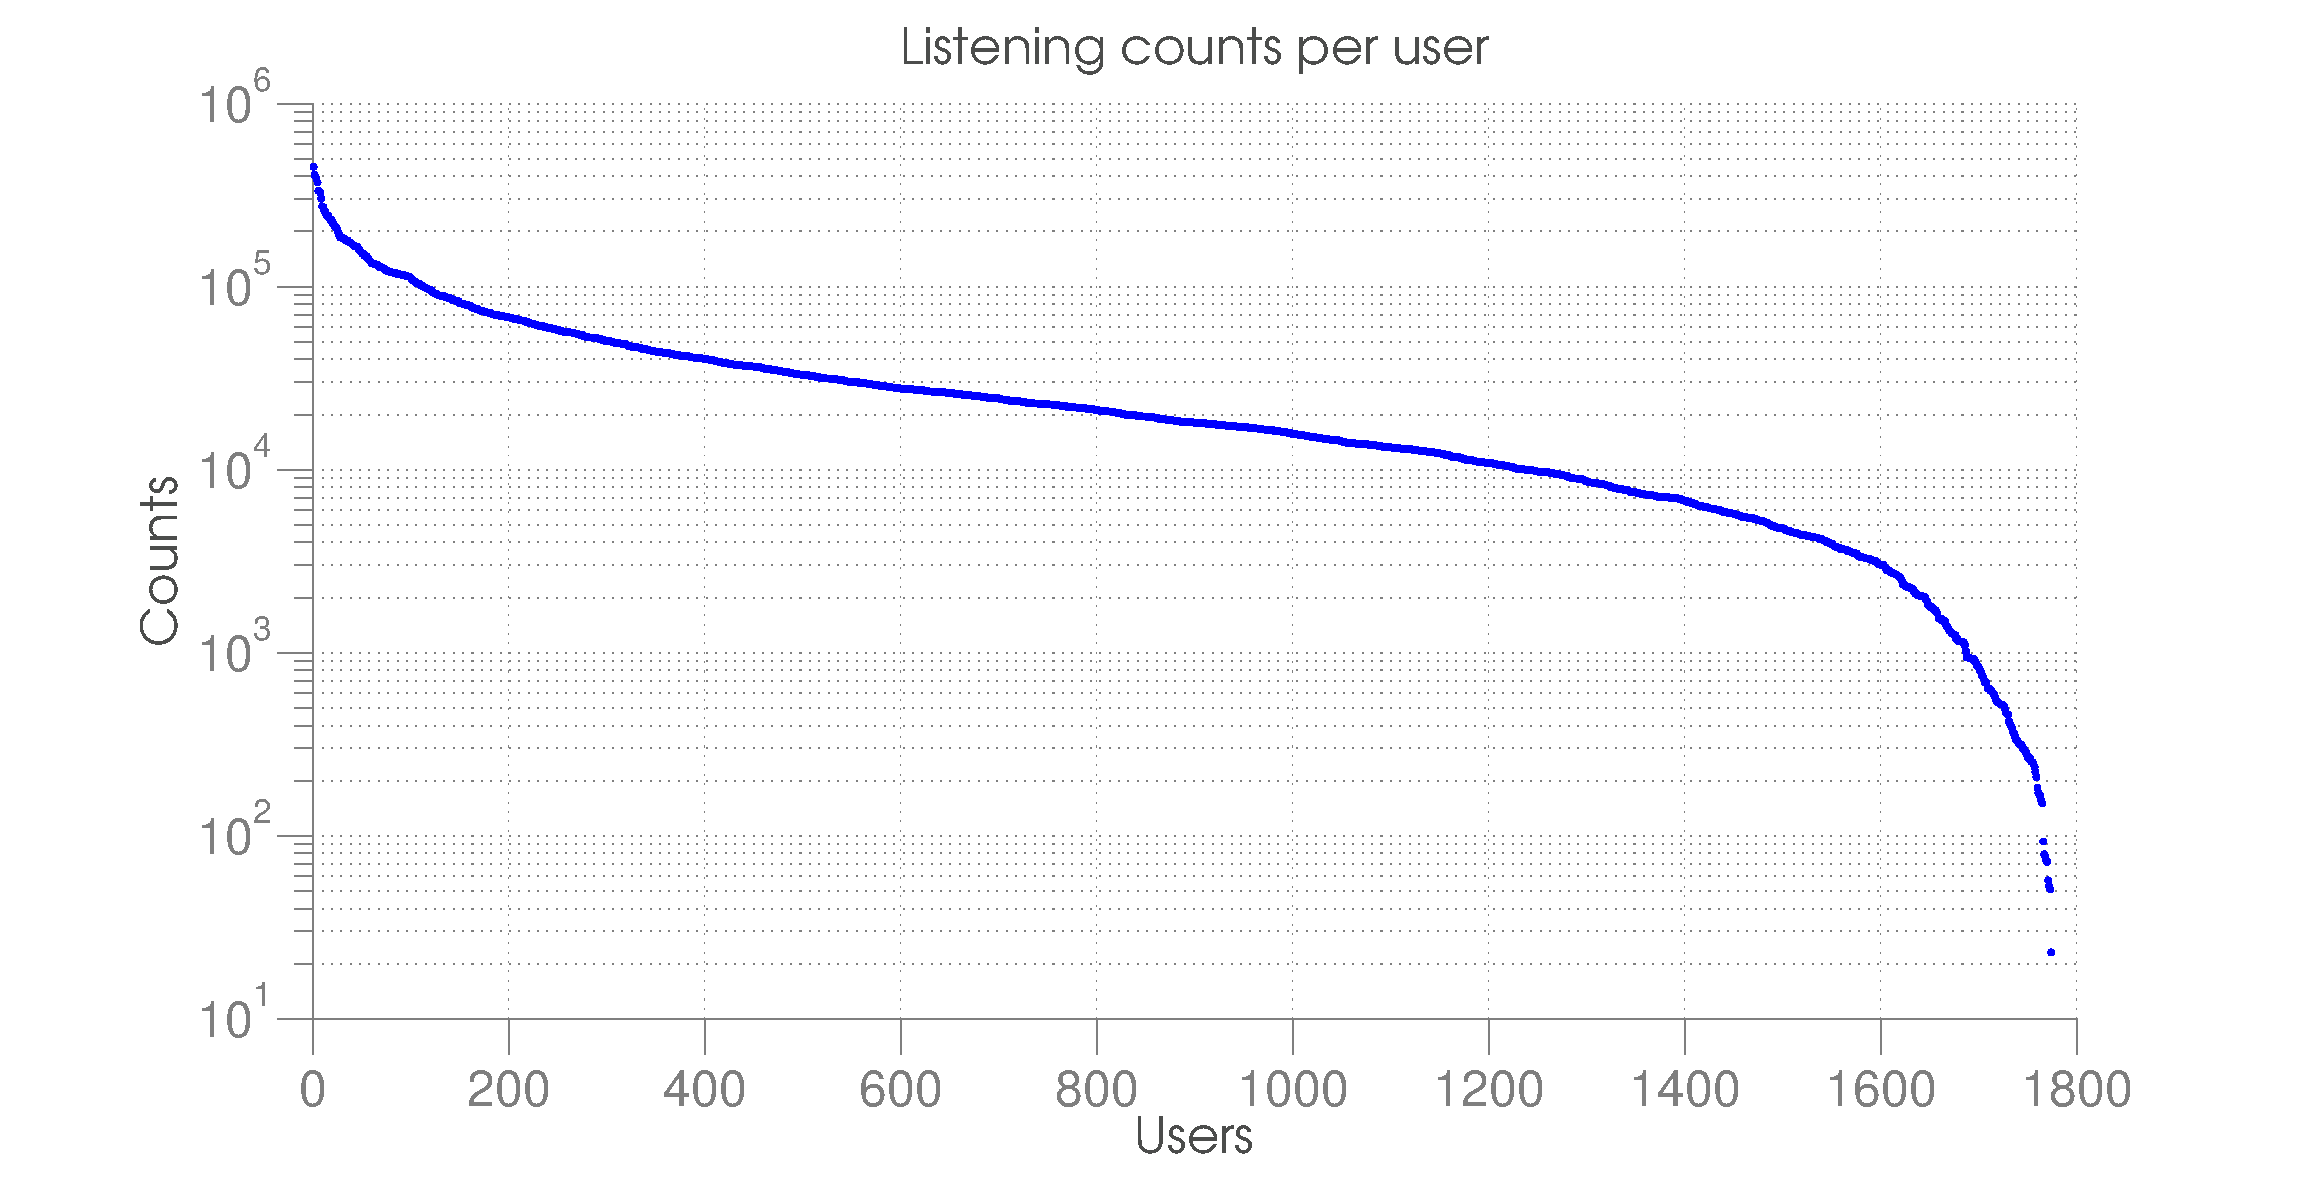
\includegraphics[trim=0mm 0mm 18mm 6mm, clip=true,
% 	width=.475\columnwidth]{figures/Counts_per_User.eps}
% 		\label{fig:listenCounts}}
% 	\hfill
% 	% trim option's parameter order: left bottom right top
% 	\subfigure[Distribution of ratings in the training set after transformation.
% 	We can see that it looks almost normally distributed.]
% 	{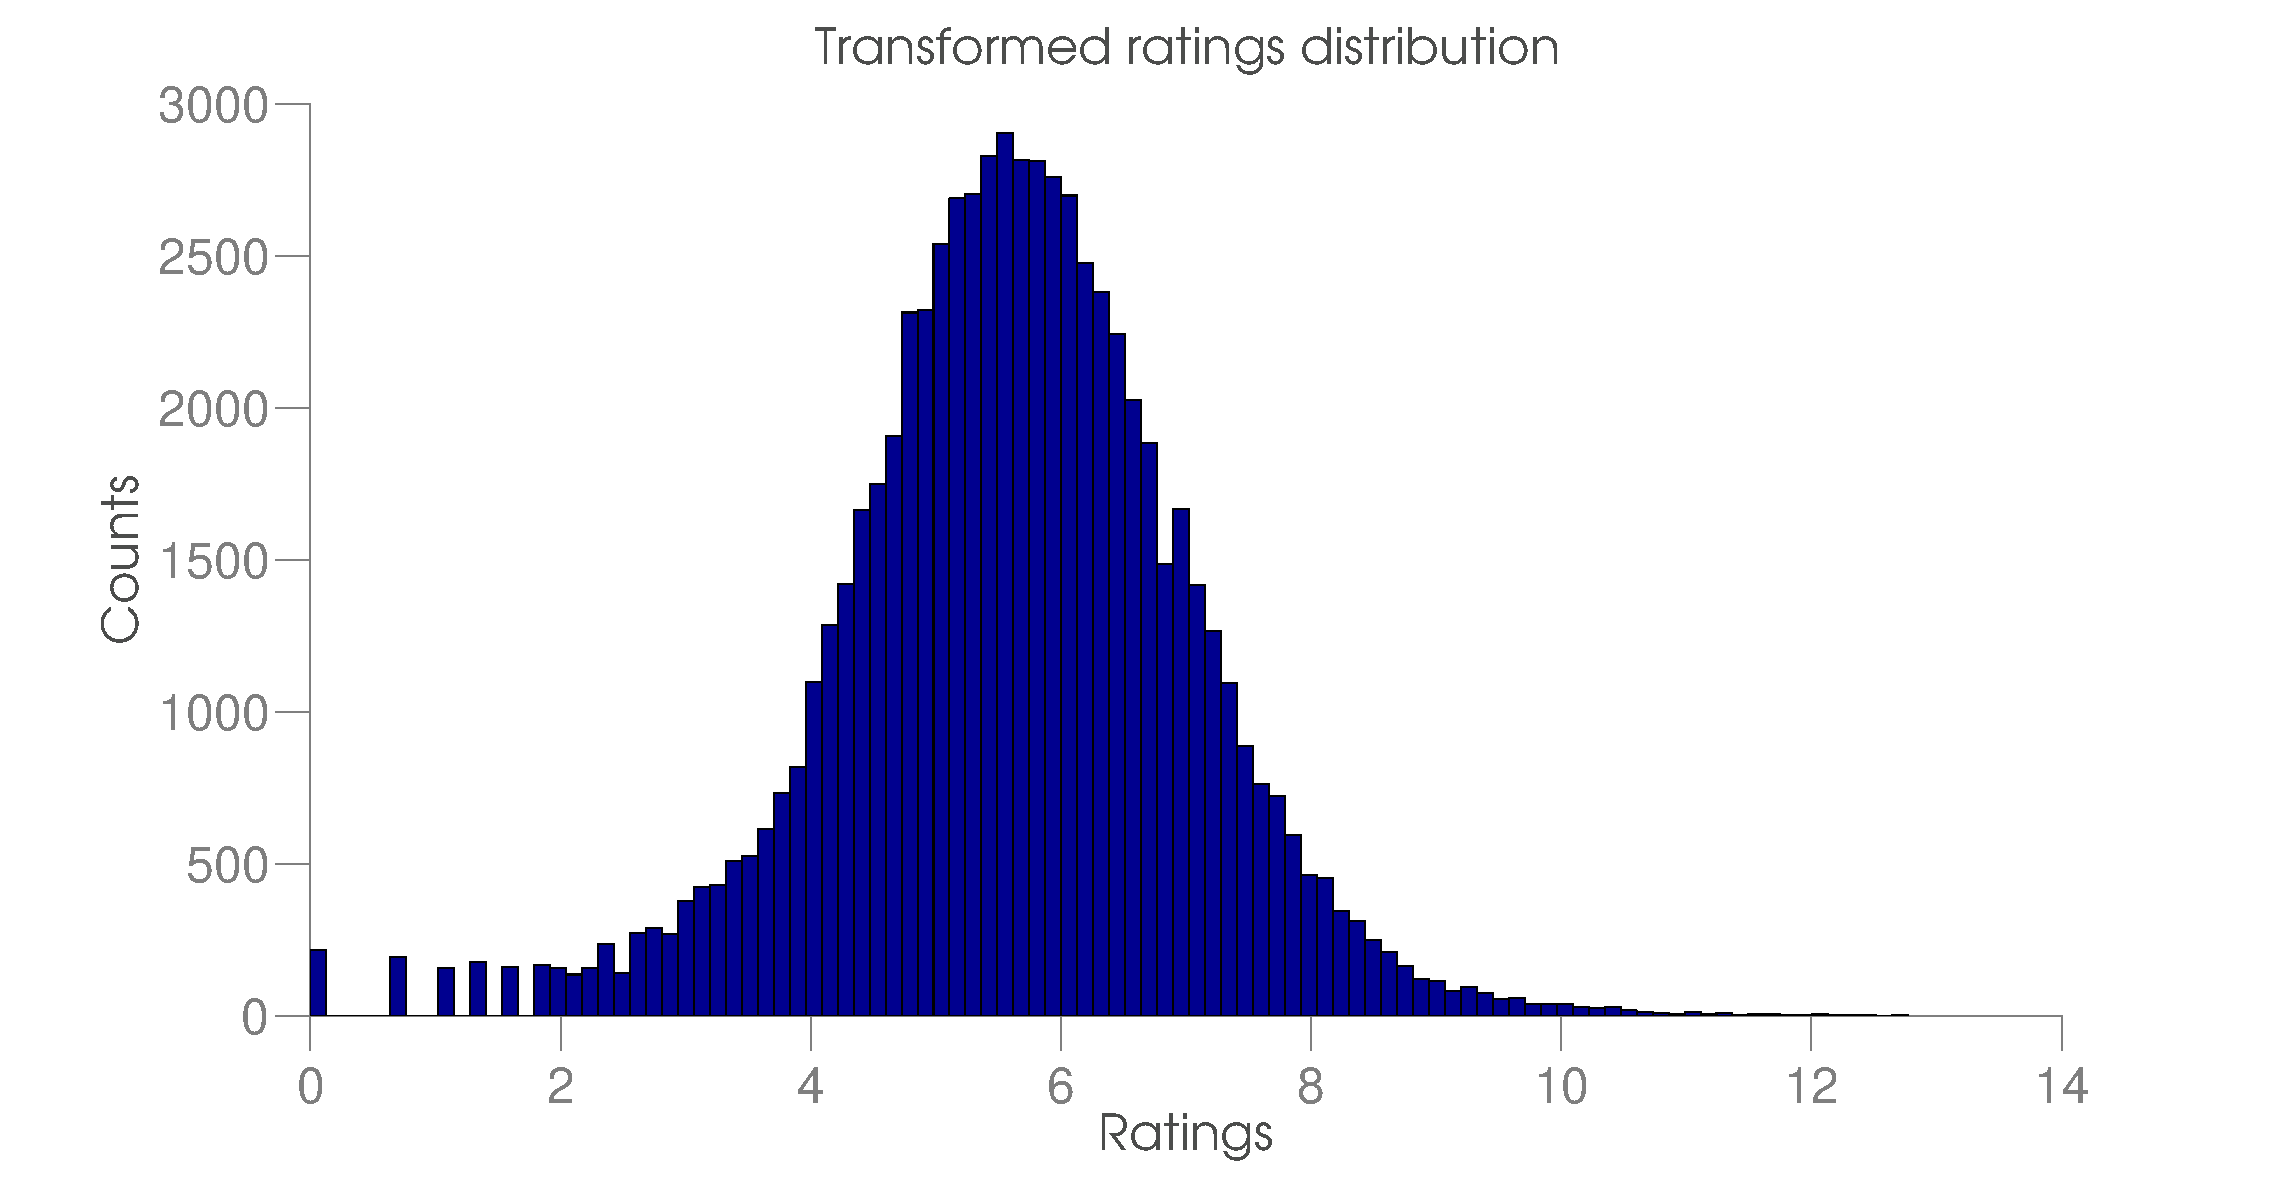
\includegraphics[trim=0mm 0mm 18mm 6mm, clip=true, width=.475\columnwidth]{figures/Transformed_Data.eps}
% 		\label{fig:transformData}}
% 	\caption{Listening count distribution before and rating distribution after
% 	data transformation}
% \end{figure}


As statistics above indicates, and as we have verified by plots, listening
counts for users, for items and friendship counts follow the power law. (omited
due to lack of space)
Computing RMSE on values that are different by the orders of magnitude can lead
to inacurate evaluation, therefore RMSE was actually computed on the log scale.
Additionally, many algorithms either assume that ratings are normally
distributed, or are converging faster under these assumptions. Therefore, we
decided to log-transform the data and work only with the transformed data. We
tried using Box-Cox transformation $X' = {X^{\lambda} - 1 \over \lambda}$,
but optimal lambda was very small, giving result almost equal to $log(X)$. 

% We also
% tried transforming all ratings for each user onto 0-1 scale independently, but
% results were worse than with log transform. Figure \ref{fig:transformData}
% shows the distribution of all ratings in the training set after the transformation.

\subsection{Models-Andrii}

In the following subsections we present three groups of models we applied.
Most of the approaches we tried are collaborative filtering. However, item
average-based model can be viewed as a simplest case of content-based filtering.
We employ the following notation: $R$, $I$, $U$ - set of all ratings,
items(artists) and users in the training set, $R(i)$ - set of all ratings for
item $i$, $R(u)$ - set of all ratings for user $u$, $r_{u,i}$, $\hat{r_{u,i}}$ -
real and predicted rating for the item $i$ by user $u$. $G_{u,v}$ - 0 or 1
depending on whether $v$ is a friend of $u$.

\subsubsection{Baseline-Andrii}

Baseline models try to generate prediction without exploiting user or item
similarity. We try different combinations of global average, average per
user and average per item approaches.

$\bm{Avg_G}$: $\hat{r_{u,i}} = \bar{r} \equiv {\sum_{r \in R}r \over |R|}$ -
global average;

$\bm{Avg_{G+U}}$: $\hat{r_{u,i}} = \bar{r_u} \equiv \bar{r} +  {\sum_{r \in
R(u)}(r - \bar{r}) \over |R(u)|}$ - global + user average;

$\bm{Avg_{G+I}}$: $\hat{r_{u,i}} = \bar{r_i} \equiv \bar{r} +  {\sum_{r \in
R(i)}(r - \bar{r}) \over |R(i)|}$ - global + item average;

$\bm{Avg_{G+U+I}}$: $\hat{r_{u,i}} = \bar{r} + \bar{r_u} + {\sum_{r \in R(i)}(r
- \bar{r} - \bar{r_u}) \over |R(i)|}$ - global + user + item average;


% \begin{enumerate}
%   \item 
% $\hat{r_{u,i}} = \bar{r} \equiv {\sum_{r \in R}r \over |R|}$ - global average;
%   \item
% $\hat{r_{u,i}} = \bar{r_u} \equiv \bar{r} +  {\sum_{r \in R(u)}(r - \bar{r})
% \over |R(u)|}$ - global + user average;
%   \item
% $\hat{r_{u,i}} = \bar{r_i} \equiv \bar{r} +  {\sum_{r \in R(i)}(r - \bar{r})
% \over |R(i)|}$ - global + item average;
%   \item
% $\hat{r_{u,i}} = \bar{r} + \bar{r_u} + {\sum_{r \in R(i)}(r - \bar{r} -
% \bar{r_u}) \over |R(i)|}$ - global + user + item average;
% 
% \end{enumerate}


\begin{figure}[!t]
	\center
	\subfigure[Distribution of ratings in the training set after transformation.
	We can see that it looks almost normally distributed.]
	{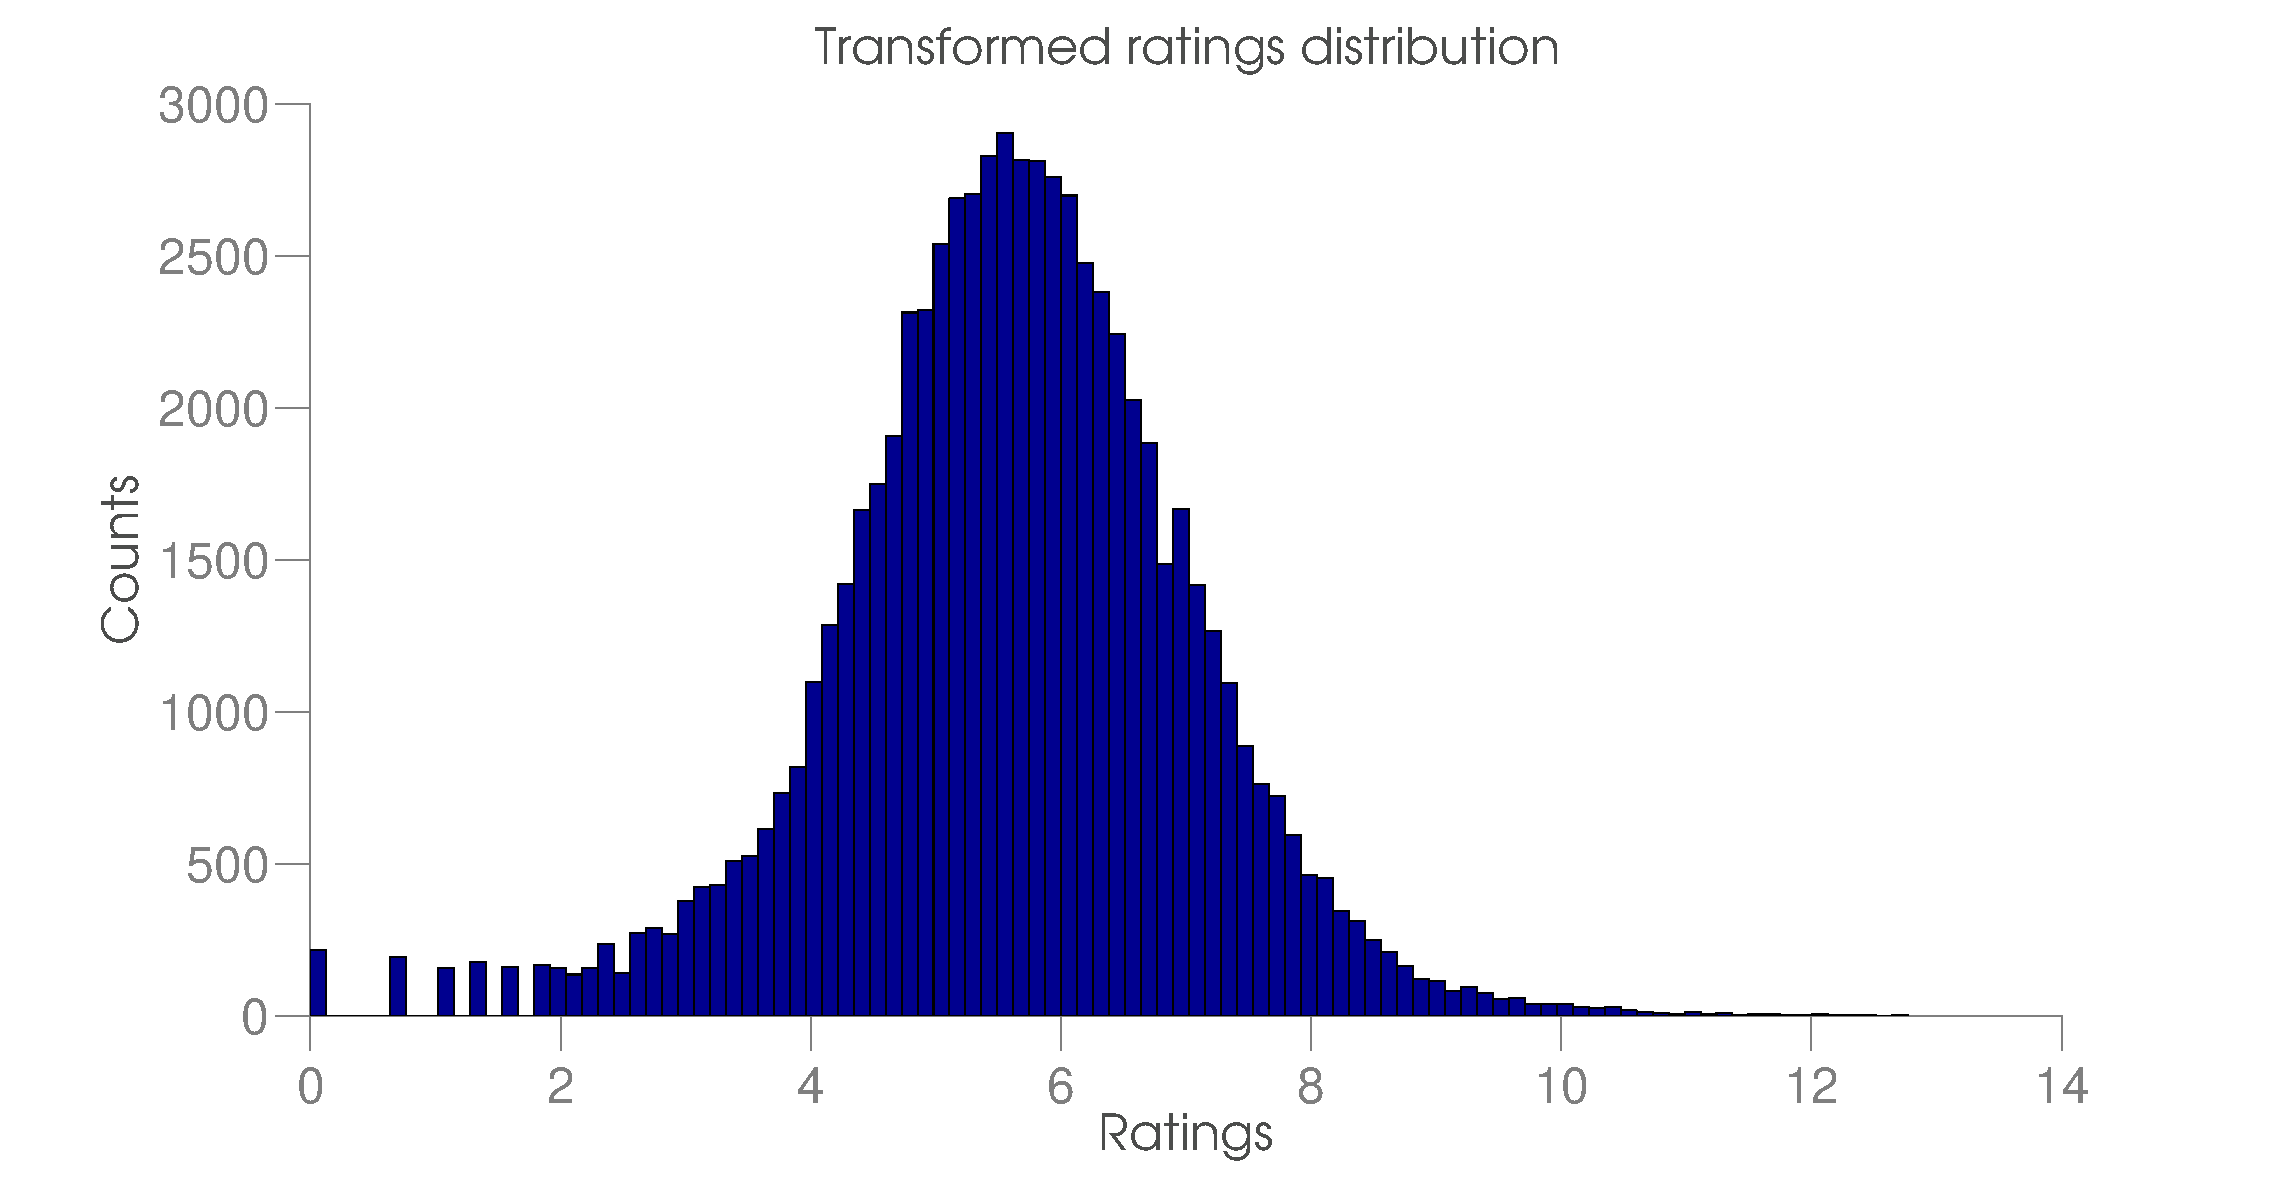
\includegraphics[trim=0mm 0mm 18mm 12mm, clip=true,
	width=.475\columnwidth]{figures/Transformed_Data.eps}
		\label{fig:transformData}}
	\hfill
	 	\subfigure[Train and test RMSE for weak generalization as a function of the
 		number of latent factors in ALS (with and without friendship).]
 		{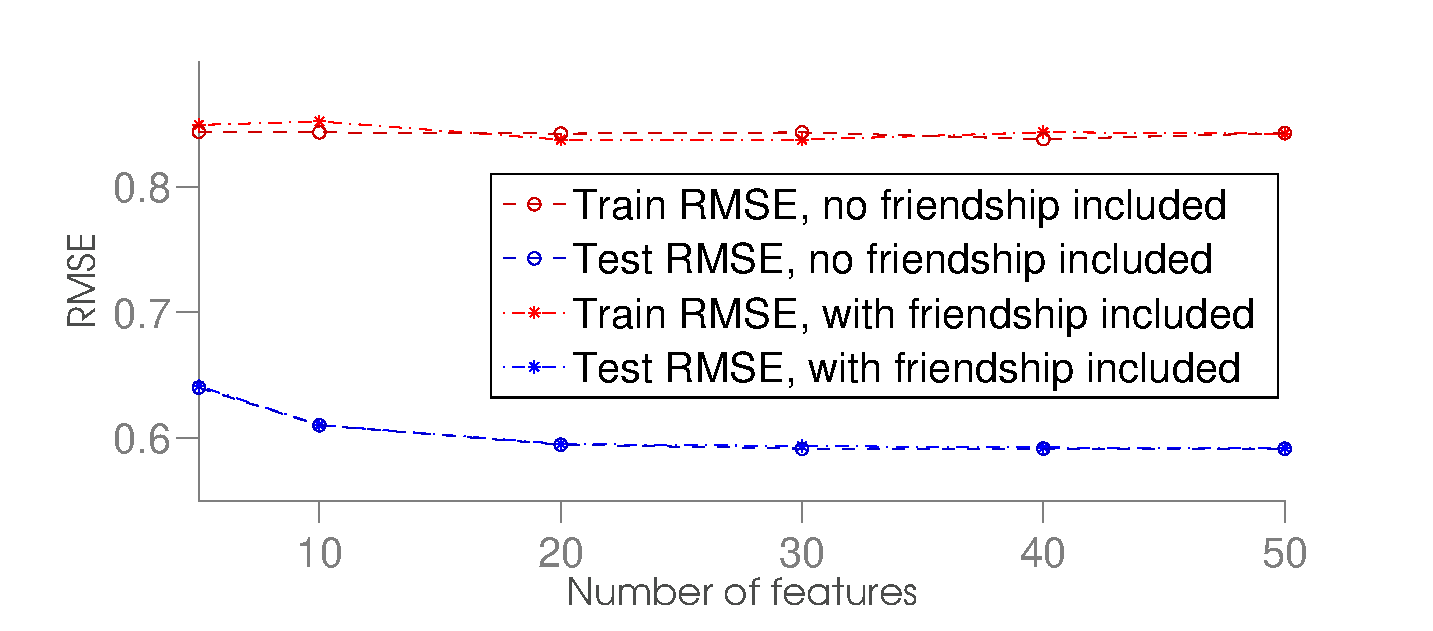
\includegraphics[trim=0mm 0mm 18mm 6mm, clip=true,
 		width=0.475\columnwidth]{figures/LatentFactors/LatentFactors2.eps}
 		\label{fig:LatentFactors}}
 	\caption{Left: Transformed ratings distribution; Right: RMSE vs number of
 	latent factors in ALS}
	% trim option's parameter order: left bottom right top	
\end{figure}


Careful extraction of baseline predictors
is important since all other approaches are applied on the data, from which
these predictors were subtracted.(\citep{bell2007lessons}) If we don't subtract
them, similarity between users is harder to detect (e.x. if two users have similar ratings for all items
that differ by one, subtracting user average will make their ratings equal and
help spot their similarity). As it turned out, more complex methods described
below were always performing worse than the baseline if we did not subtract
baseline from them, therefore for all algorithms below we subtracted the
averages, computed predictions and then added baseline prediction.

\subsubsection{Matrix factorization techniques-Igor}

Some of the most successful realizations of latent factor models for recommender 
systems are based on matrix factorization\citep{bell2007lessons}. We assume
that all users and all items are characterized by vectors of factors. Matrix factorization learns the 
latent characteristics which are used to generate predictions $\hat{r_{u,i}}$. 
There are few different matrix factorization techniques. Zhou et al. \cite{zhou2008large} have
successfully applied ALS-WR (Alternating-Least-Squares with Weighted-lambda-regularization) to the Netflix dataset. 
The optimization problem can be defined as:

\begin{equation}\label{eq:one}
f(U, M)=\sum_{\left ( i,j \right )\in R} \left ( r_{i,j} -
\mathbf{u}^{T}_{i}\mathbf{m}_{j} \right )^{2}+\lambda \left ( \sum_{i}|R(i)|
\left \| \mathbf{u}_{i} \right \| ^{2} + \sum_{j}|R(j)|\left \| \mathbf{m}_{j}
\right \| ^{2} \right )
\end{equation}


We have included the friendship graph by adding the following term to $f(U, M)$:

\begin{equation}\label{eq:test}
f^{*}(U, M)=f(U, M)+\lambda
_{T}\sum_{i}(\mathbf{u}_{i}-\frac{1}{f_{i}}\sum_{v}G_{i,v}\mathbf{u}_{v})
\end{equation}

where $f_{i}$ denotes the number of friends of user $i$. 
This integration of the friendship information have been used in \cite{jamali2010matrix}. The
model can be made more complex if we add bias and if we assign different importance 
factor for each $\hat{r_{u,i}}$. The latter is important if we have non-Gaussian data like in our case. 
However, our goal is to generate relevant predictions in the log domain where the predictions are Gaussian 
and that is why we can use formula \eqref{eq:test}. 
We also didn't include the bias in our ALS models because 
we substracted it from the data before running the model.

In both cases rating prediction is computed as follows: $\hat{r_{i,j}} =
\mathbf{u}_{i}^T \times \mathbf{m}_{j}$. We will refer to our algorithm as
$\bm{ALS}$ when the results are produced by optimizing \eqref{eq:one}, and as
$\bm{ALS_F}$ when using \eqref{eq:test}.

\subsubsection{Neighbourhood-based methods-Andrii}

Neighbourhood-based methods try to explore similarity between users or items. We
explored the similarity between users, as we had additional information in the
form of friendship graph. In the general case, weighted nearest neighbour
methods estimate rating as follows:
$\hat{r_{u,i}} = {{\sum_{v \in N(u)}w_{u,v} * r_{v,i}}\over \sum_{v \in
N(u)}w_{u,v}}$. $N(u)$ is defined in the terms of some number of items $v$ with
highest similarity $Sim_{u,v}$. We assumed $w_{u,v} = Sim_{u,v}$. We also tried
setting $w_{u,v} = 1$, but performance was worse, so we omit these variations.

$\bm{KNN_C}$: $Sim_{u,v} = {\sum_{i \in I}r_{u,i} * r_{v,i} \over \sqrt{\sum_{i
\in I}{r_{u,i}^2} * \sum_{i \in I}{r_{v,i}^2}}}$ - cosine similarity. This is the
  only approach that employs ratings given by user $u$ and is therefore only
  suitable for weak generalization. Neighbourhood is defined at $k$ items
  with the highest similarity, $k$ is selected using cross-validation.
  
$\bm{KNN_S}$: $Sim_{u,v} = {1 \over D_{u,v}}$, $D_{u,v}$ is the shortest path in
the friendship graph between nodes $u$ and $v$, or $\infty$ if none exists.
Neighbourhood is defined in the same way as in previous approach.

$\bm{KNN_{S2}}$: Variation of the previous approach, where we consider only
nodes with distance less than 3 (since we have a quite dense graph and shortest distances
rarely are greater than 6). In this and all approaches below, we experimentally
found out that we get best results when we include all nodes into the
neighbourhood of each node (majority of nodes have 0 similarity and do not
affect the rating prediction) - limiting the size of the neighourhood means not
taking into consideration some of the nodes with non-zero similarity. This also
frees us of necessity to tune the size of the neighbourhood.

$\bm{KNN_F}$: $Sim_{u,v} = G_{u,v}$. We average over all friends of the user.
This can also be seen as a variation of a previous approach where we only consider
nodes with distance 1.

$\bm{KNN_P}$: $Sim_{u,v} = PR(v) * G_{u,v}$, $PR(v)$ is sum of
  $v$-th row of $(I - G * D)^{-1}$, where $D_{i,j}$ is 1 divided by indegree of
  $j$. This is an attempt to weigh friends of the node by their relative
  ``importance'' - their PageRank with damping factor of 1.
  For more details and explanation of damping factor, please see
  \cite{page1999pagerank}.

% \begin{enumerate}
%   \item $Sim_{u,v} = {\sum_{i \in I}r_{u,i} * r_{v,i} \over \sqrt{\sum_{i \in
%   I}{r_{u,i}^2} * \sum_{i \in I}{r_{v,i}^2}}}$ - cosine similarity. This is the
%   only approach that employs ratings given by user $u$ and is therefore only
%   suitable for weak generalization. The optimal $k$ for this algorithm can be
%   selected by cross-validation.
%   \item $Sim_{u,v} = G_{u,v}$. In order to always have all friends of user in
%   the neighbourhood, we set $N(u)$ to have all friends of user $u$. This also
%   frees us of tuning $k$.
%   \item $Sim_{u,v} = {1 \over D_{u,v}} * G_{u,v}$, where $D_{u,v}$ is the length
%   of the shortest path in the friendship graph between nodes $u$ and $v$ or infinity,
%   if no path exists.
%   \item Variation of \#3 where only nodes at distance 1 and 2 are
%   considered (since most pairs of nodes have distance less than 6, only close
%   nodes are considered)
%   \item $Sim_{u,v} = PR(v) * G_{u,v}$, where $PR(v)$ is the ``importance'' of
%   node $v$, computed as its PageRank with damping factor 1: $PR(v)$ is sum of
%   $v$-th row of $(I - G * D)^{-1}$, where $D_{i,j}$ is 1 divided by indegree of
%   $j$.
% \end{enumerate}

Interesting note about the friendship graph-based methods is that they perform
better when we average also over 0es in the ratings of friends, instead of
omiting them. While in general 0s indicate missing information, we assume that
if some of the friends of the user listened to the artist, and others didn't,
that indicates that they know and don't like this particular artist. We
attribute better success of averaging over all friends to this fact.


\subsection{Results}

\subsubsection{Parameter tuning}


% \begin{figure}[!t]
% 	%\center
% 	\subfigure[Learning curve for the model KNN.] 
% 		{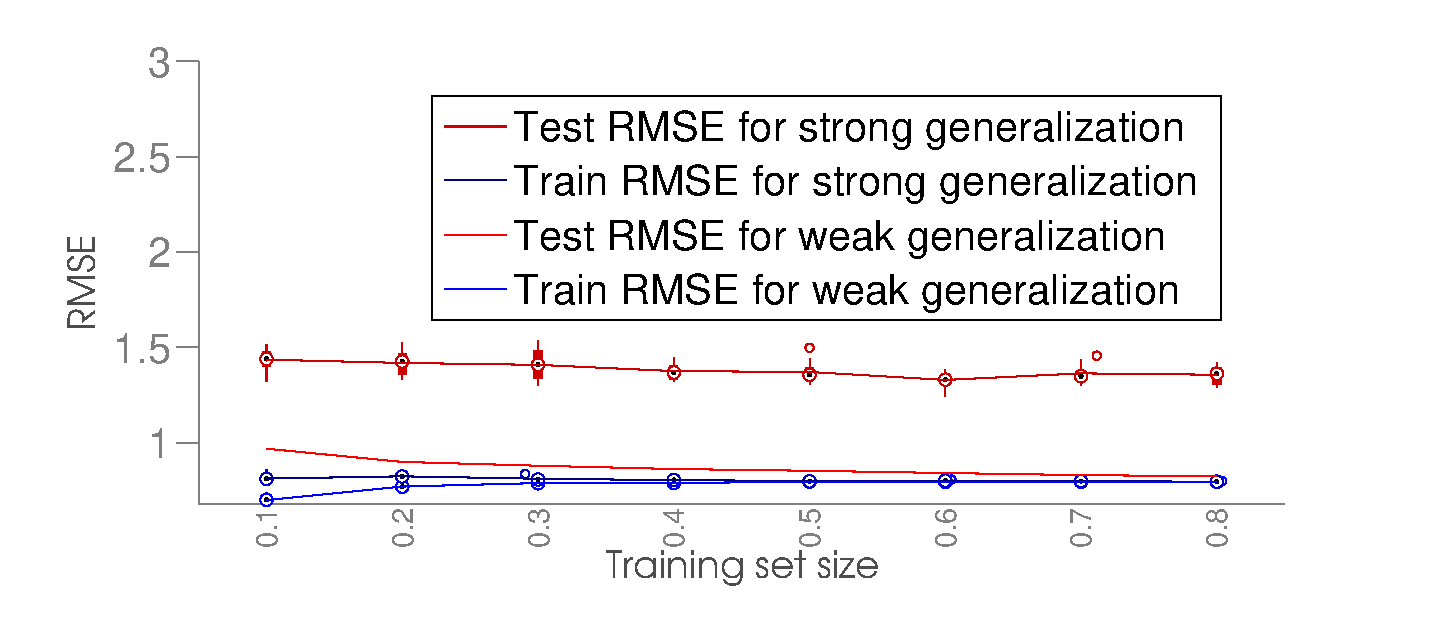
\includegraphics[trim=0mm 0mm 18mm 6mm, clip=true,
% 		width=0.475\columnwidth]{figures/LearningCurveCombined/LearningCurveCombined2.eps}
% 		\label{fig:LearningCurveCombined}}
% 	\hfill
% 	% trim option's parameter order: left bottom right top
% 	\subfigure[Train and test RMSE for weak generalization as a function of the
% 		number of latent factors in ALS (with and without friendship).]
% 		{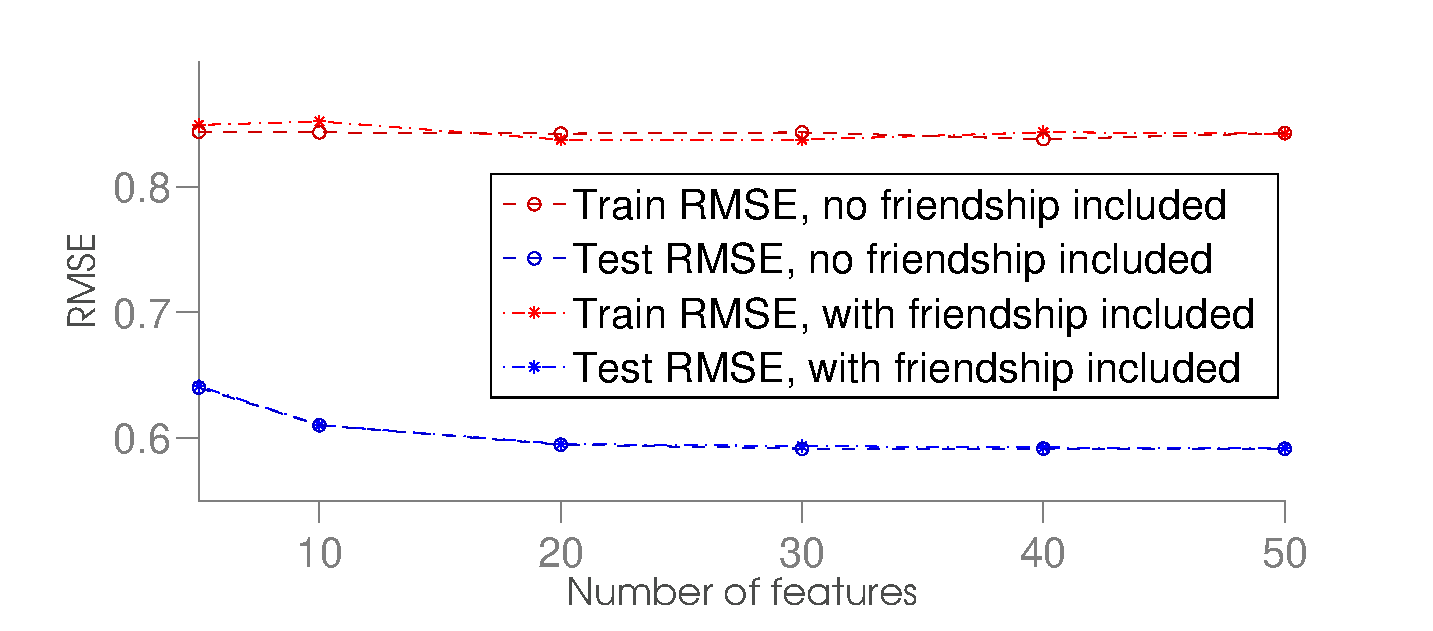
\includegraphics[trim=0mm 0mm 18mm 6mm, clip=true,
% 		width=0.475\columnwidth]{figures/LatentFactors/LatentFactors2.eps}
% 		\label{fig:LatentFactors}}
% 		\caption{Parameter tuning for ALS}
% \end{figure}

The quality of the predictions depends on the training set size. 
In the training data set there are 69617 ratings. After analyzing the learning
curve (not shown due to lack of space), we saw that RMSE continues to increase
as we increase size of the training set, up to maximum. Therefore, we decided to
use the heldout set of the size, equal to the size of the test set (on relative
scale) - 20\% for weak generalization and 5\% for strong. In all our
cross-validations, we used 10 random splits with the appropriate size of the
held-out set.

 
 We used such cross-validation to choose
 the optimal value of $\lambda=0.2$ for fixed number of latent factors. Using
 small number of latent factors might not cover all characteristics of the 
 data and using large number of latent factors might lead
 to overfitting. 
 The quality of the model also depends on $\lambda$ and $\lambda_{T}$ (if we
include the social graph in the model).
To reduce model complexity we have set $\lambda=\lambda_{T}$ [3].  
 We have observed that 30 iterations are enough to obtain convergence of the learning process. 
 In Fig.\ref{fig:LatentFactors} we can see the train and test error for 
 different number of latent factors in ALS (with and without friendship) with $\lambda=0.2$. 
 We need to emphasize that before running ALS we substract the baseline and in the 
 end we add the baseline back. If we don't do this, ALS cannot reach to the baseline solution.




%    In ALS we calculate the vector of factors $\mathbf{u}_{i}$ for the new user $i$ as an average 
%    of the vectors of factors associated with her/his friends. 
%    In KNN we calculate $\hat{r_{u,i}}$ as an average rating given to the item $i$ by the friends of $u$.
%    When none of the friends has rated the item, the algorithm outputs the global average 
%    as estimate of $\hat{r_{u,i}}$. In contrast to KNN, ALS could produce user specific 
%    predictions $\hat{r_{u,i}}$ even if the friends of $u$ have not rated the item $i$. 
%    However, KNN proved to be better in practice.


\subsubsection{Methods comparison}


% \begin{figure}[!t]
% 	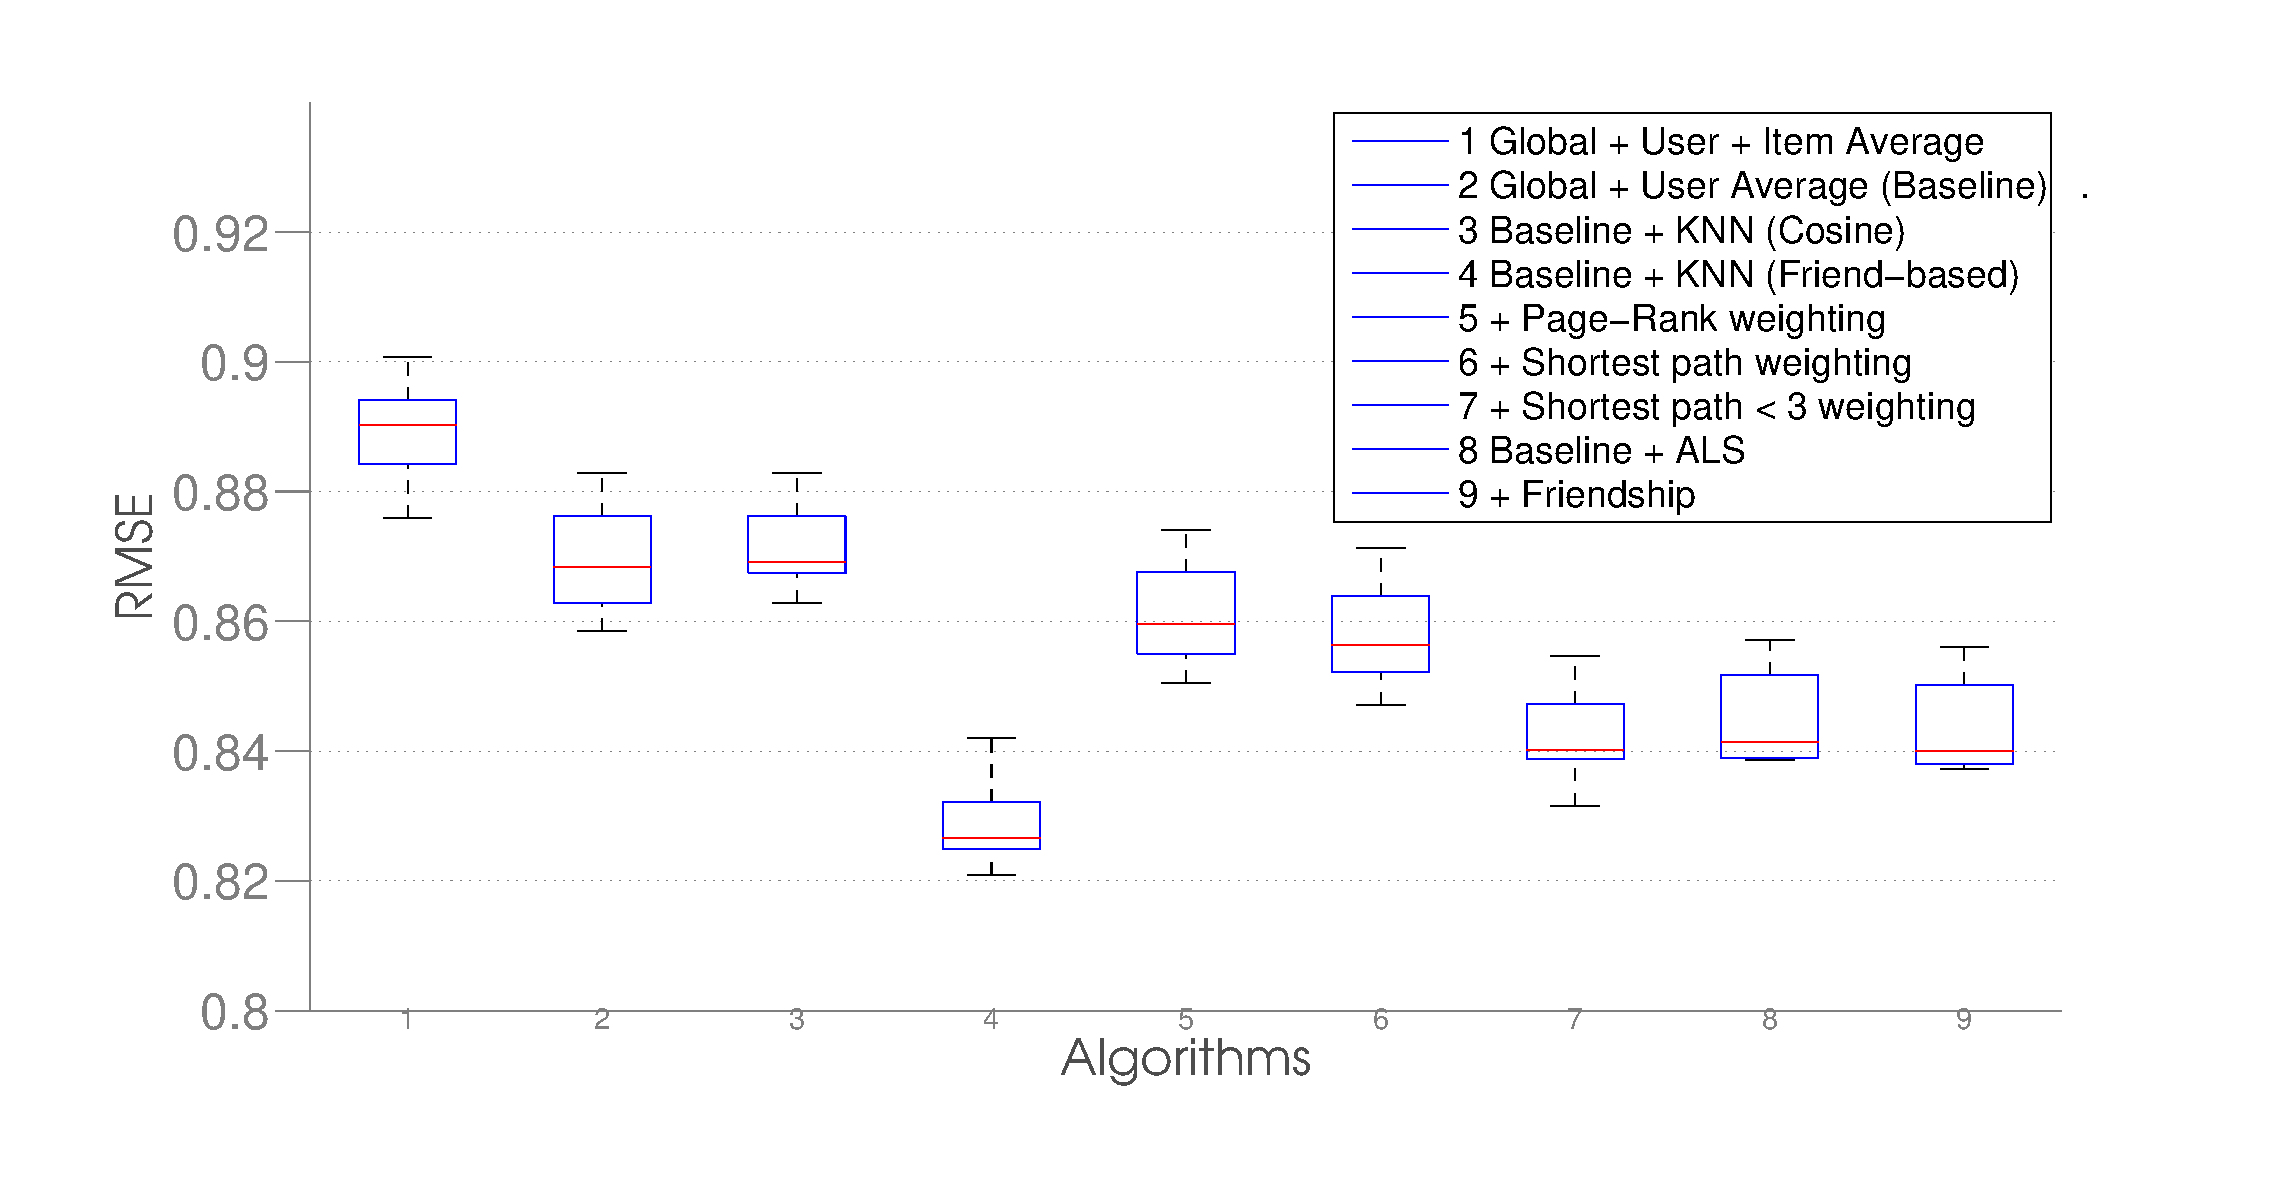
\includegraphics[trim=0mm 0mm 18mm 6mm, clip=true,
% 	width=.9\columnwidth]{figures/Algorithms_Weak.eps}
% 	\caption{Performance of different algorithms for weak generalization task}
% 	\label{fig:algorithmsWeak1}
% \end{figure}
 

Table \ref{table:Algorithms} shows performance of different algorithms for both
strong and weak generalization task. Results were obtained by 10-fold cross
validation on the training set. In all cases standard deviation was quite small
compared to the mean of the prediction (never exceeding 0.03) and we decided to
omit it to save space. For strong generalization task for methods that can't
deal with cold start problem results are equal to the results of $\bm{Avg_G}$ and were omited.

First observation that we can make is that computing average over items makes
performance worse, which computing average over items makes it better. We
assume, that there is no strong signal in the average of item ratings since
different users can listen to the same artists number of times that differ by
orders of magnitude - but there is more uniformity in the ratings from one user.
We selected $\bm {Avg_G}$ as baseline for strong generalization and
$\bm{Avg_{G+U}}$ for weak.

\begin{table}[!t]
\hspace*{-1cm}
\bgroup
%\def\arraystretch{0.8}
\setlength{\tabcolsep}{.16667em}	
\begin{tabular}{| c | c | c | c | c | c | c | c | c | c | c | c |}
\hline
Task, Dataset & $Avg_G$ & $Avg_{G+U}$ & $Avg_{G+I}$ & $Avg_{G+U+I}$ & 
$KNN_C$ & $KNN_S$ & $KNN_{S2}$ & $KNN_F$ & $KNN_P$ & $ALS$ & $ALS_F$ \\ \hline
  Strong, Testing & 1.4272 & --- & 1.4728 & --- & --- & 1.3990 & 1.3905 &
 \textbf{1.3854} & 1.4010 & ---- & 1.3885 \\ \hline
 Weak, Testing & 1.4517 & 0.8699 & 1.5858 & 0.8900 & 0.8717 & 0.8581 & 0.8426 &
 \textbf{0.8294} & 0.8615 & 0.8455 & 0.8443 \\ \hline
 %Weak, Training & 1.3910 & 0.8359 & 1.2223 & 0.7298 & 0.8354 & 0.8248 & 0.8095
 % & 0.7974 & 0.8273 & 0.5923 & \textbf{0.5917} \\ \hline
\end{tabular}
\caption{Performance of different algorithms for different tasks}
\label{table:Algorithms}
\egroup
\end{table} 
 

We can see that all other methods perform better than baselines. We see that for
ALS-based methods adding friendship into the model improves performance, but not
much. In both tasks best overall method is $\bm{KNN_F}$, and other KNN-based
methods go in the order: $\bm{KNN_{S2}}$, $\bm{KNN_S}$ (optimal neighbourhood
size $k$ selected by cross-validation - 100), $\bm{KNN_P}$, $\bm{KNN_C}$($k$ =
55).
We can explain poor performance of $\bm{KNN_C}$ and good performance of simple
$\bm{KNN_F}$ by the lack of data - more complex method requires more data.
Indeed, on the training set the lowest error was achieved by $\bm{KNN_C}$ and $\bm{ALS_F}$, 
but they didn't achieve lowest test error - a sign of
overfitting of complex models and lack of training data. 


% Figure \ref{fig:algorithmsWeak1} shows peformance of different algorithms for
% weak generalization task. Two algorithms with much worse results were omited:
% The global average ($RMSE=1.4517 \pm 0.0093$) and global + item average ($RMSE=1.5858 \pm 0.009$).
% Comparison of these two results, as well as global + user average and global +
% user + item average shows that algorithms actually perform worse when we try to
% subtract item averages - but slightly better when we subtract user averages. We
% assume that reason for that is the fact that for one artist listening counts
% from different users often differ by the orders of magnitude and there us no
% strong signal that we could extract from that. However, such signal is present
% in user average.
% Further inspection of the graph shows that all other algorithms perform better than baseline. This is expected as they
% subtract the baseline first. Out of KNN-based algorithms, simple
% friendship-based KNN performs best, surpasing shortest-path based methods,
% followed by PageRank-based and cosine similarity-based (for it, K was selected
% using 10-fold cross-validation and was equal to 100).
% For ALS-based methods, we see only a small improvement in performance when frienship is included in the
% model. Interestingly, for KNN-based methods, performance on the training set
% (not shown because of the lack of space) is better for more complex models,
% while being worse on the test set - a sign of overfitting and lack of training
% data.


% \begin{table}
% \center
% \begin{tabular}{| p{1.3cm} | p{1.6cm} | p{2cm} | p{2cm} | p{1.5cm} | p{1.6cm}
% | p{1cm}|}
% \hline
% Algorithm Dataset & KNN: Friendship & KNN: Shortest paths $<3$ & KNN: Shortest
% paths & KNN: PageRank & ALS: Friendship & Average \\ \hline
% 
% Training & $0.7967$  & $0.8097$ & $0.8266$ & $0.8296$ & \textbf{0.6278} &
% $1.4021$ \\ \hline
% 
% Testing &  \textbf{1.3854} & $1.3905$ & $1.399$ & $1.4010$ & $1.3885$ &
% $1.4272$ \\ \hline
% \end{tabular} 
% \caption{Performance of different algorithms for strong generalization
% task}
% \label{table:AlgorithmsStrong}
% \end{table}


% For the task of strong generalization, we omited 4 of the algorithms used for
% weak generalization, that are not suited for strong generalization. For the
% rest, ordering of algorithms was almost the equal to the ordering for weak
% generalization: the worst is baseline (global average), with testing error of 
% $1.4272 \pm +0.009$, followed by page-rank based KNN (1.4010), KNN with shortest
% paths (1.399), KNN with shortest paths shorter than 3 (1.3905), ALS with
% friendship (1.3885) and, finally, friendship-based KNN (1.3854). In all cases,
% standard deviation was very low compared to the mean RMSE itself, and we omited
% it.

% For the task of strong generalization, we omited showing global + user average
% algorithms, KNN + cosine similarity, and ALS without friendship algorithms, as
% they use previous ratings of the user and in this case just return 0 prediction.
% Here, again, KNN with friendship information obtained the best result, being by
% small margin better than ALS + friendship. Other KNN-based methods performed
% worse, probably due to small amount of data and high noise.

To generate our final predictions in both strong and weak generalization task
we used KNN with friendship, computed after subtracting a baseline. As we
mentioned in the algorithm description, we averaged all ratings of friends of
the user, including zeros. If we averaged over only positive ratings, we
got results worse than baseline (0.9602 for weak and 1.4897 for strong
generalization).


% \begin{figure}[t!]
% 	\center
% 	% trim option's parameter order: left bottom right top
% 	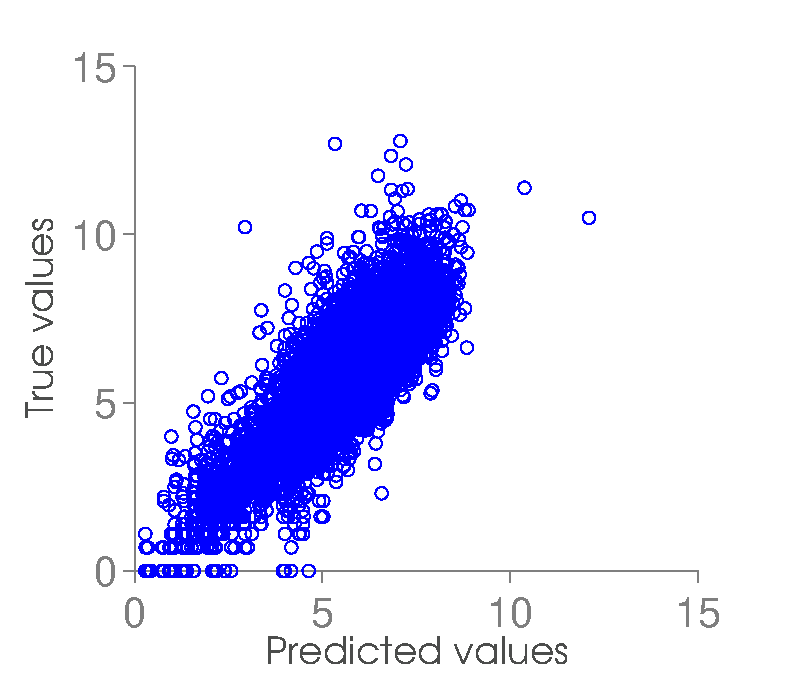
\includegraphics[trim=0mm 0mm 0mm 0mm, clip=true, scale=0.5, width=0.5\columnwidth]{figures/PredictedTrue/PredictedTrueSmall.eps}
% 	\caption{}
% 	\label{fig:PredictedTrue}
% \end{figure}
% 

\subsubsection{Prediction quality}

\begin{figure}[!t]
	\center
	\subfigure[Predicted values obtained using KNN vs. true test values.] 
	{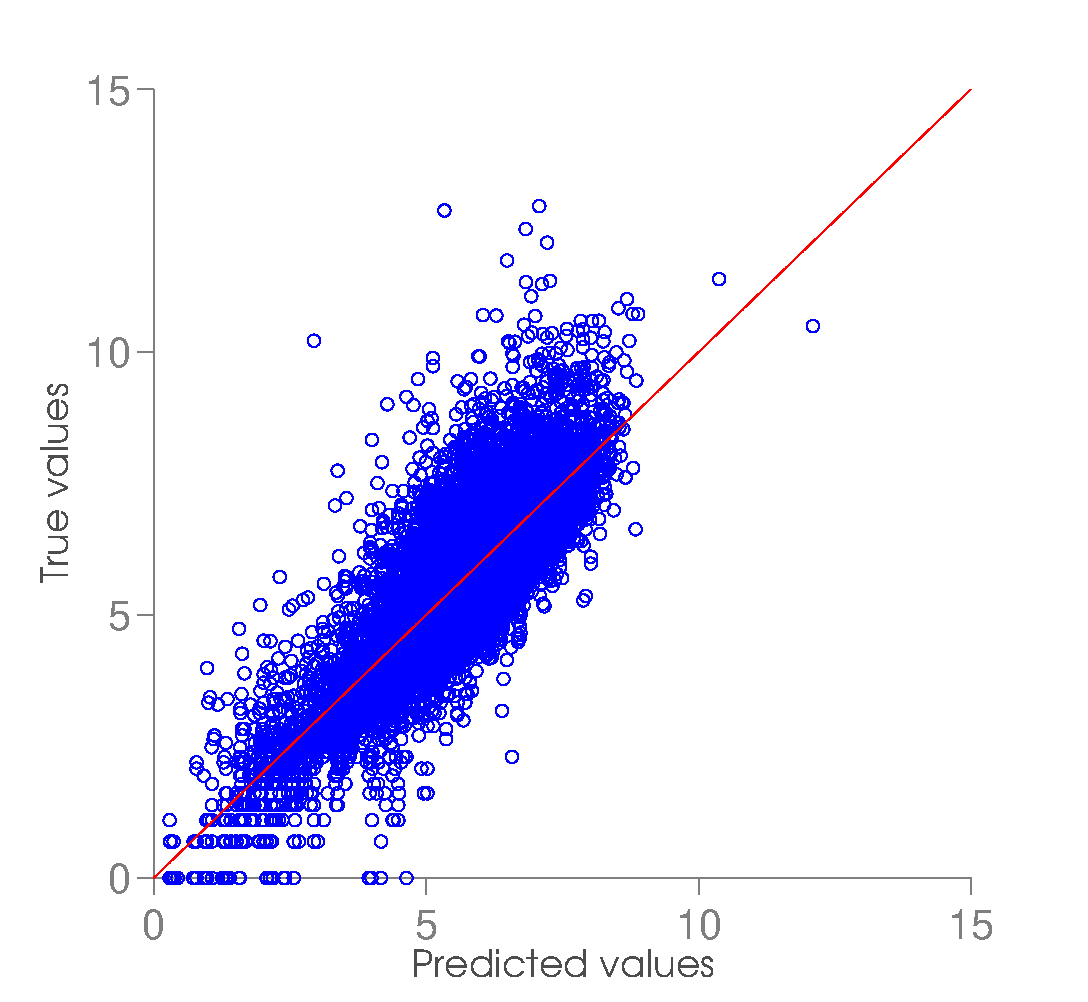
\includegraphics[trim=0mm 0mm 6mm 10mm, clip=true,
	width=.35\columnwidth,height=4cm]{figures/PredictedTrue/PredictedTrueLarge2.eps}
	\label{fig:PredictedTrue}}
	\hfill
	% trim option's parameter order: left bottom right top
	\subfigure[Average absolute error for a number of unique users per artist and
	artists per user.] {\includegraphics[trim=0mm 0mm 6mm 3mm, clip=true,
	width=.55\columnwidth,height=4cm]{figures/Heatmap.eps}
		\label{fig:heatmap}}
	\caption{Left: True vs Predicted values; Right: Average error for different
	user / item categories}
\end{figure}

To verify that our algorithm performs slightly better than random, we have
plotted the real and predicted values of ratings in Fig.\ref{fig:PredictedTrue}
for our best approach, $\bm{KNN_F}$.
In ideal case, all points should appear on the $y=x$ line. 
In our case, the points are distributed around the main diagonal and their distribution is Gaussian, 
just like the distribution of ratings in the test set, but we see a strong
correlation between our predictions and true values. We can see that error is
bigger when we try to predict higher ratings. We tried to
investigate this relationship by looking at how our algorithm performs for
different categories of users and items, for weak generalization.
We sorted and broke down
sets of all users and artists into 5 equal parts, depending on the number of
unique artists user has listened to, and to the number of unique users who listened to the particular item.
We calculated average value of absolute prediction error in each of the 25 parts
and interpolated the results for all the other points of the space. Figure
\ref{fig:heatmap} shows the result. As we can see, our best approach performs
best for users that have rated a lot of artists, and these artists are listened
to almost exclusively by those users. Also, not surprisingly, worst results are
for the users who have only rated a few most popular artists - predicting their
(high!) ratings is a difficult task. We haven't found any
dependence of performance on the number of friends of a users.

\section{Person detection problem}

The second task of this project is people detection from images. The goal is to predict which images contain 
a person, and which do not. In essence it is a binary classification problem which we have tried to tackle 
with Sparse Logistic Regression (SLR) and k-Nearest Neighbors (kNN) classifiers.
The quality of the classification is evaluated by the Receiver Operating Characteristic (ROC) curve. == ADD  ABOUT 10 pow -2 wjflwekfjkl 10 pow -3

%  In addition, we 
% have employed input feature transformations such as Principal Component Analysis (PCA), 
% t-Distributed Stochastic Neighbor Embedding (t-SNE) and Fisher Vectors (FV). In the following text, 
% we explain our approach in more detail.

\subsection{Data Description}

The training data for the pedestrian detection consists of 8545 images, of which 
1237 are positive samples, i.e. they contain a person, and 7308 are negative samples. 
With each image we also receive its feature vector, more precisely the Histogram of 
Oriented Gradients (HOG) feature vector, and its label (binary). Each feature vector 
has dimensionality of $D$ = 9360.

The test dataset consists of 8743 samples. Here we receive only the HOG descriptor for each image.
 The goal is to train a classifier by using
the training data, which will assign a probability to each test feature vectors of it belonging to 
the positive class. 

%<Correlation plot. Pedestrian vs. non-pedestrian.>(FIGURE)

\subsection{Data transformation}

The input dimensionality $D$ of the HOG descriptors is very large. 
Since our data set is not very large, we believe that the useful 
signal in the data can be conveyed in much less dimensions. 
In addition, the high dimensionality of the features increases 
the training time of each classifier, and we suspect that 
it might also lead to the curse of dimensionality.
 For dimensionality reduction we have used two methods: PCA and t-SNE.

\begin{figure}[!t]
	\center
	\subfigure[Dimensionality reduction using PCA] 
	{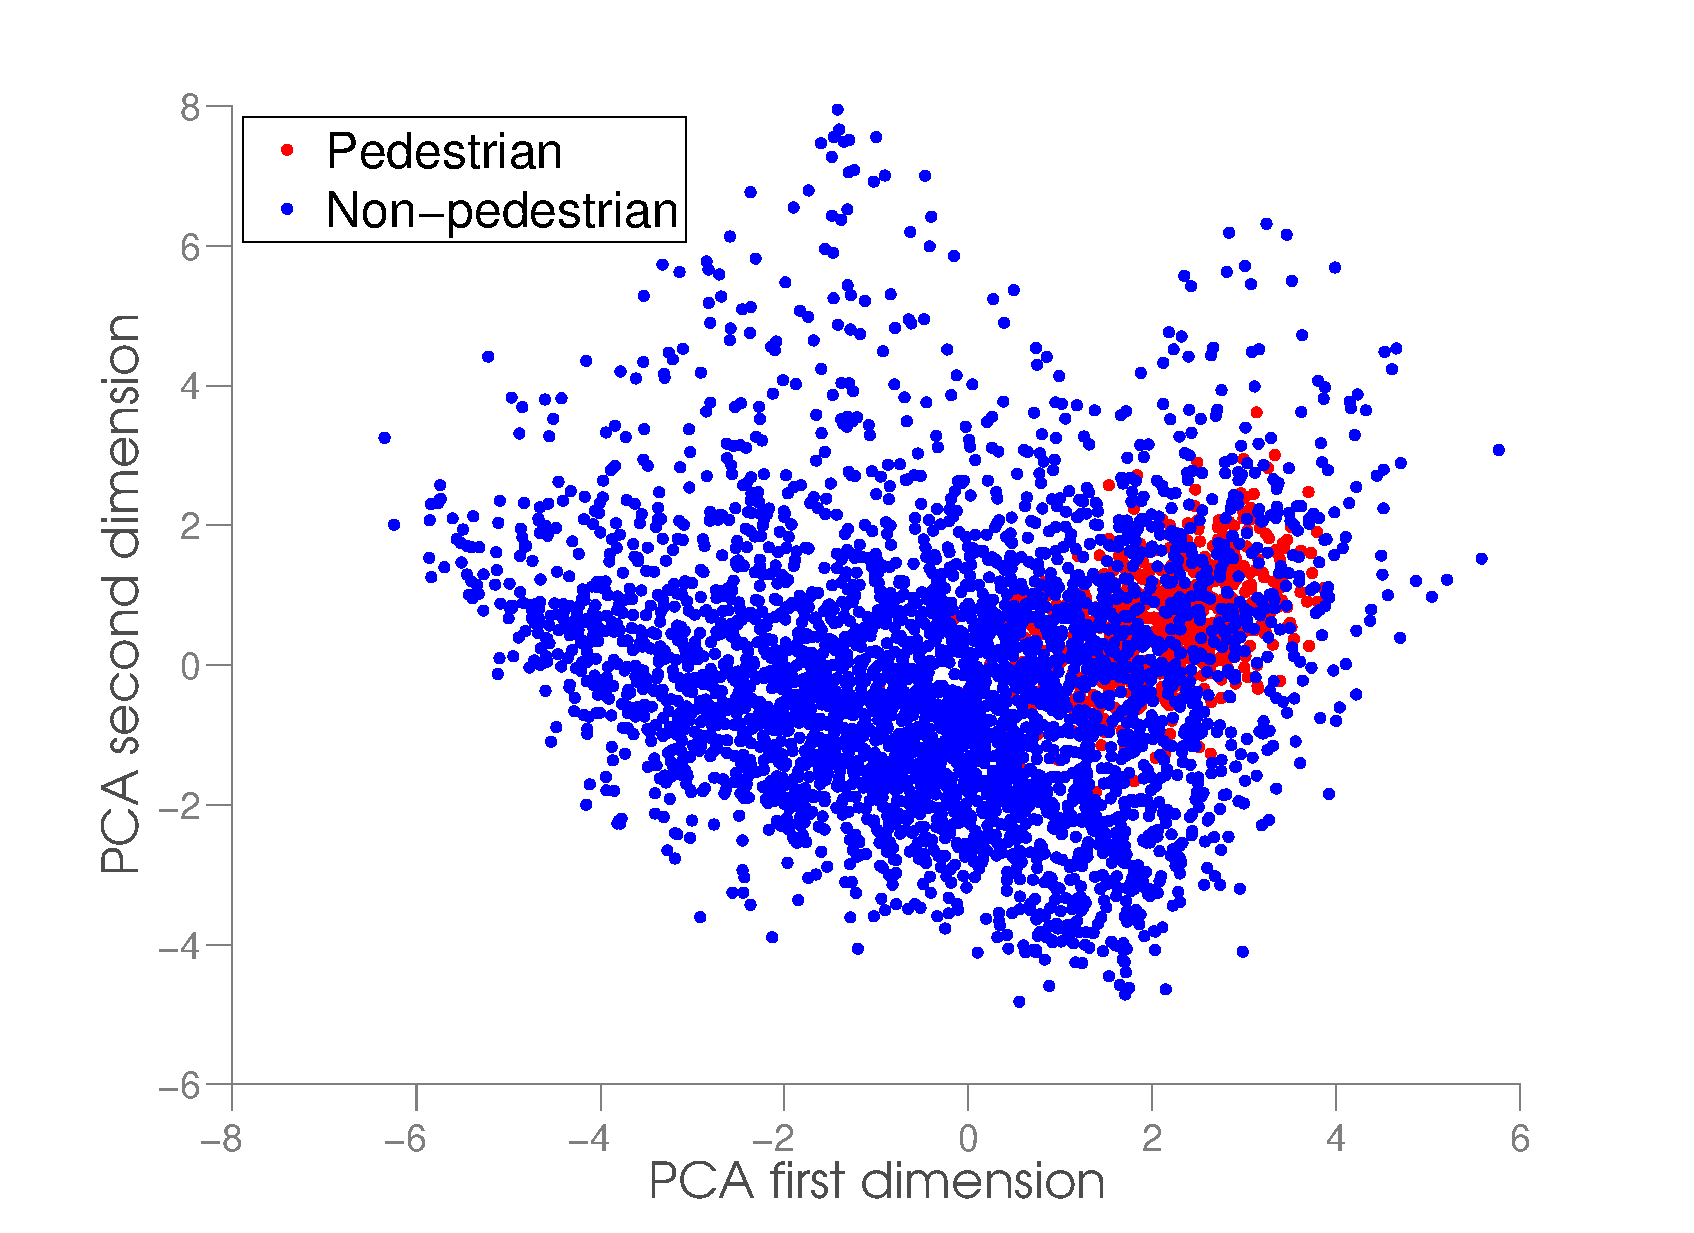
\includegraphics[trim=0mm 0mm 6mm 15mm, clip=true,
	width=.475\columnwidth,height=4cm]{figures/PCA_mapping.eps}
	\label{fig:PCA}}
	\hfill
	% trim option's parameter order: left bottom right top
	\subfigure[Dimensionality reduction using t-SNE] {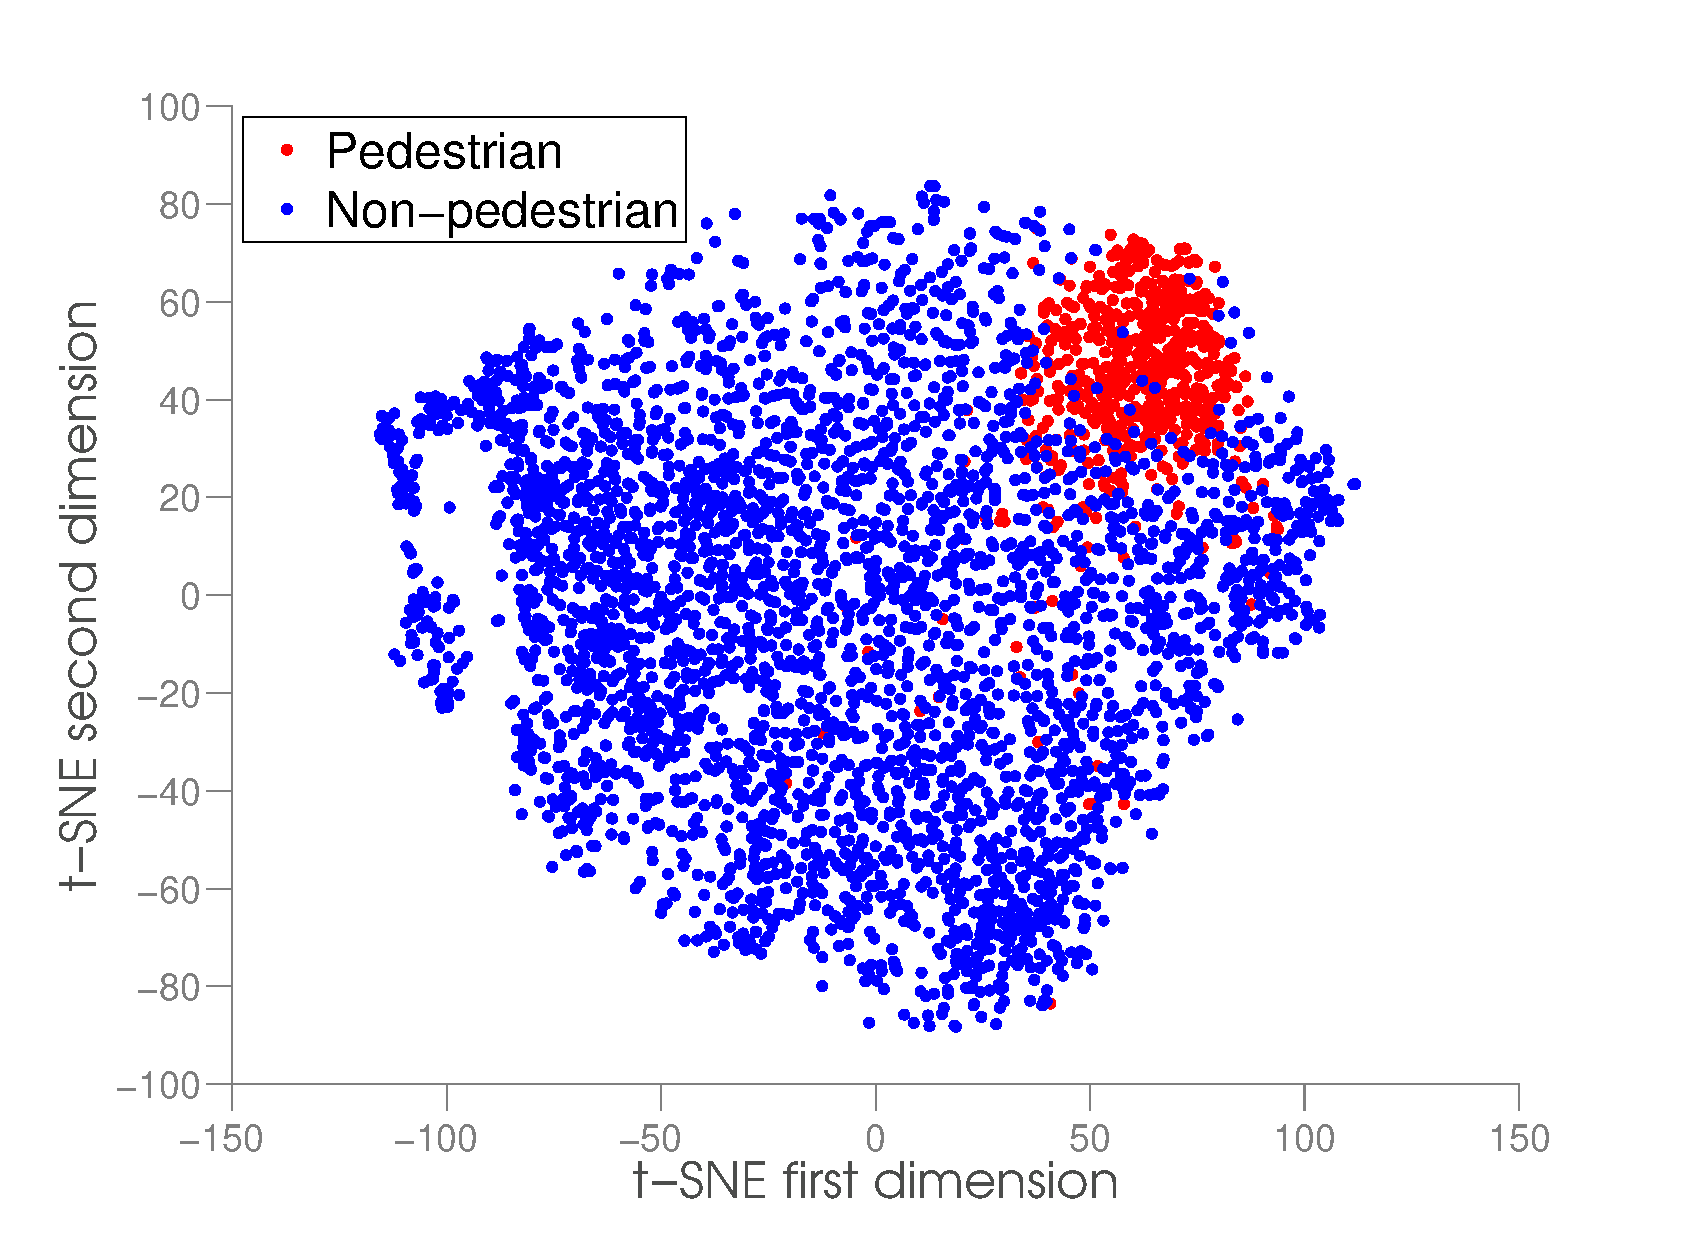
\includegraphics[trim=0mm 0mm
	6mm 15mm, clip=true,
	width=.475\columnwidth,height=4cm]{figures/t-SNE_mapping.eps}
		\label{fig:TSNE}}
	\caption{Dimentionality reduction to 2 dimensions using PCA and t-SNE}
\end{figure}


% For the purpose of dimensionality reduction we applied two different techniques
% - principal component analysis and t-distributed stochastic neighbor
% embedding(t-SNE). Their short overview is below.

\subsubsection{PCA-Andrii}

	
PCA is a dimensionality reduction technique which approximates matrix of data
$X$. First, singular value decomposition $X=USV^T$ is computed, where $U$ and
$S$ have orthogonal columns, and $S$ is a diagonal with singular values of $X$
on the diagonal. Then, the first $K$ rows and columns of $S$ and $V$ are selected,
as well as the first $K$ columns of $U$ and $S$. The product of such trimmed
matrices is a $N \times K$ dimensional matrix $\hat{X}$ ($N$ being the number of
data points), which minimizes the $Tr((X-\hat{X}) * (X-\hat{X})^T)$ expression. The
results of reducing dimension of our training data to 2 dimensions in shown in
Fig. \ref{fig:PCA};



\subsubsection{t-SNE-Andii}

Although t-SNE is generally viewed as a low dimensional visualization technique 
for high dimensional data, it can also be used for reducing the dimensions of 
data features to 2 or 3. After applying t-SNE to our dataset, we saw
that it groups fairly well the positive data samples, and we can apply a 
classification algorithm. The general idea of this approach is to find such 
low-dimensional embedding of points that are close in the high-dimensional 
space would be close in the low-dimensional. Closeness of two points in the high-dimensional
space $p_{ij} = {p_{i|j} + p_{j|i}\over 2 * N}$ is computed as the average of
asymmetric similarities, $p_{j|i} = {exp(-||x_i-x_j||^2 / 2 * \sigma_i^2) \over
\sum_{k \neq i}exp(-||x_i-x_k||^2 / 2 * \sigma_i^2)}$. The closeness in
low-dimensional space is computed as $q_{ij}={ (1 + ||y_i-y_j||^2)^{-1}\over
\sum_{k \neq i}(1+||y_k - y_i||^2)^{-1}} $, $y$ being coordinates in the
low-dimensional space. $y$ are found using gradient descent that minimizes the 
expression $\sum_{i \neq j}p_{ij}log({p_{ij}\over q_{ij}})$, which can be viewed 
as the distance between $p$ and $q$. The approach is described in full 
in \cite{van2008visualizing}. The result of applying t-SNE is shown on
the Fig. \ref{fig:TSNE}.


\subsubsection{Fisher Vector}

Fisher Vector (FV) encodes higher (second) order statistics compared to Bag-of-Visual-Words. 
It also uses a GMM as a basis for its computation. For a feature vector $x_t$, 
it computes the mean deviation vector $u_i^d$ for each Gaussian $i$ 
for dimension $d$ and the mean covariance deviation $v_i^d$, 
which are also weighted by the prior probability $\gamma_i(x_t)$ that 
the feature vector belonging to the Gaussian $i$:

\begin{center}
$u_i^d = \gamma_i(x_t) \dfrac{x_t^d - \mu_i^d}{(\sigma_i^d)^2}$,\quad \quad
\quad $v_i^d = \gamma_i(x_t) \left[ \dfrac{(x_t^d - \mu_i^d)^2}{(\sigma_i^d)^3} - \dfrac{1}{\sigma_i^d} \right]$
\end{center}

The FV is high dimensional because it is calculated for each Gaussian, each original dimension and 
there are two variables. The good side is that the priors are zeros for most of the Gaussians 
for a feature, and they are very sparse.

\subsection{Classification models}

After transforming the training data to a lower dimensional space, we use it to train a classifier 
which should produce the probabilities for our test samples. Our choice of classifiers went to SLR and kNN.

SLR is essentially a penalized logistic regression which uses a $mathrm{L_1}$ norm (Laplacian prior), 
instead of a $mathrm{L_2}$ norm (Gaussian prior), for the penalization. Since this prior 
is non-differentiable at the origin (because of the absolute value), it cannot be solved 
in a closed form. Therefore, smooth upper bounds are used as approximations to this error (penalty). 
With the bounds in place, the algorithm boils down to Iteratively Reweighted Least Squares (IRLS). 
An important strong point of this prior is that it encourages the weights to be sufficiently large or zeros. 
When the original features are used for classification, this plays the role of relevant feature selection. 
For more details, please read the original paper \cite{krishnapuram2005sparse}.

\subsection{Results}

\begin{figure}[!t]
	\center
	\subfigure[Learning curve] 
	{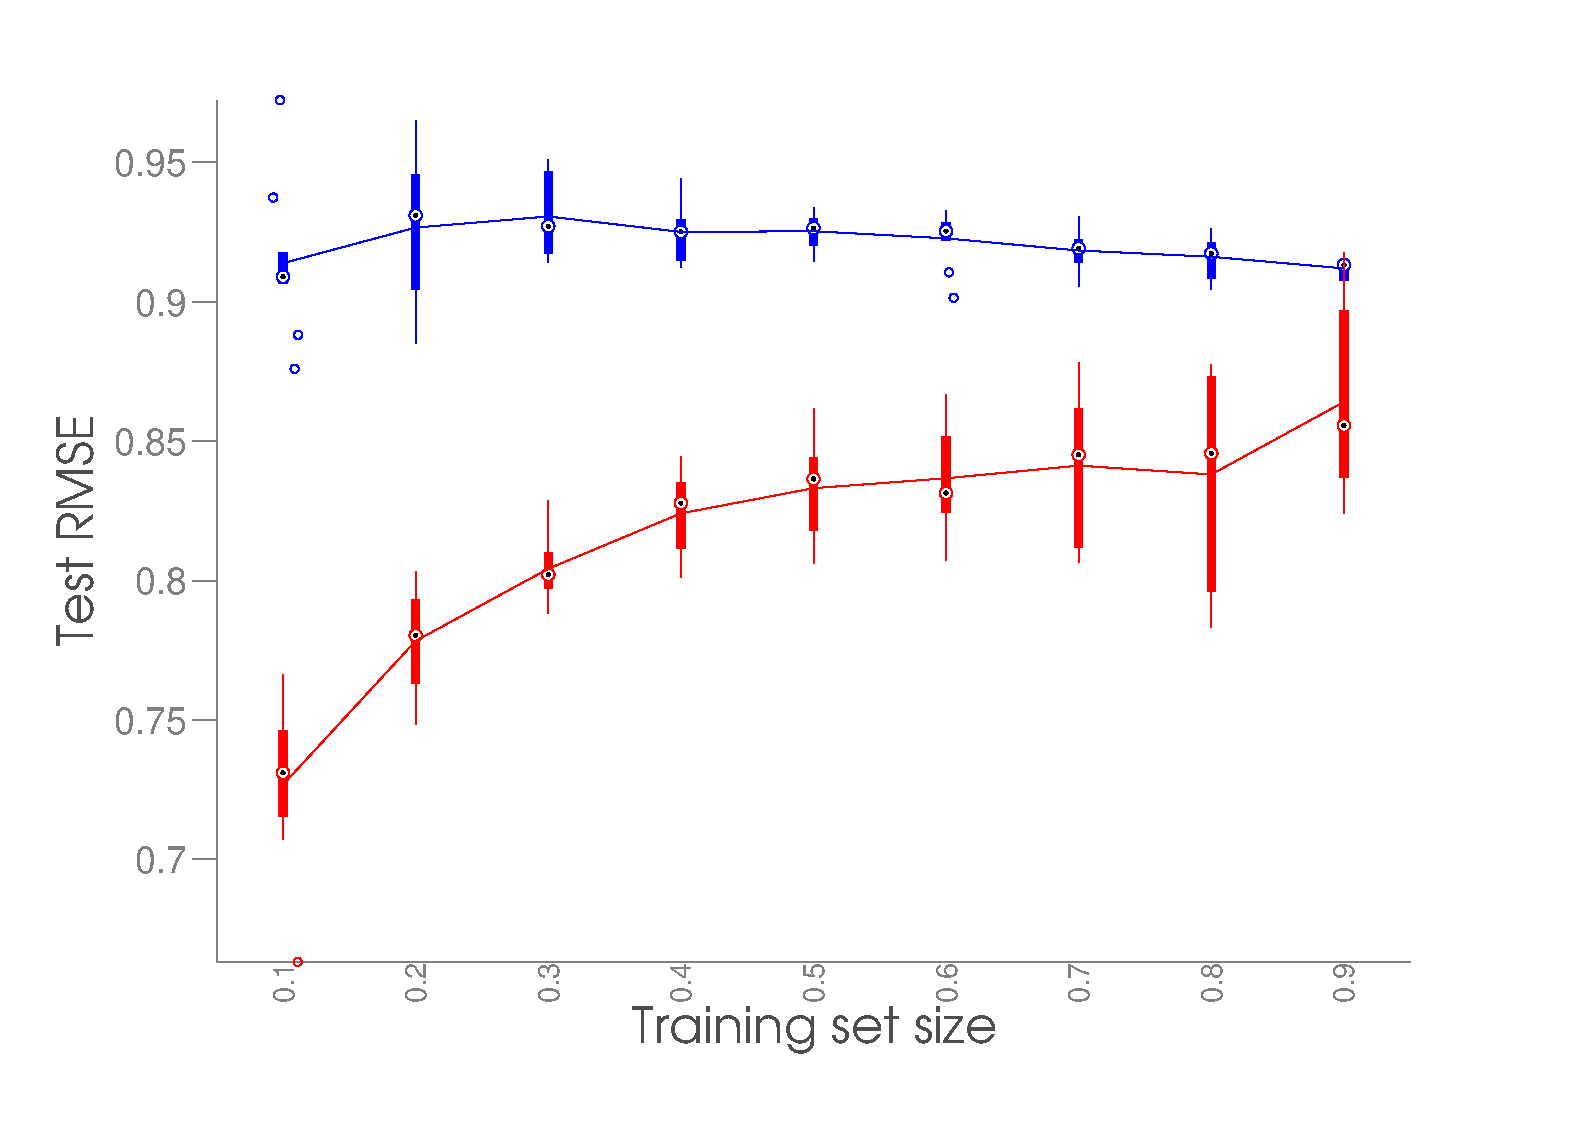
\includegraphics[trim=0mm 13mm 6mm 15mm, clip=true,
	width=.475\columnwidth,height=4cm]{figures/SMLR_learning_curve.eps}
	\label{fig:LearnCurve}}
	\hfill
	% trim option's parameter order: left bottom right top
	\subfigure[ROC curves for different algorithms] {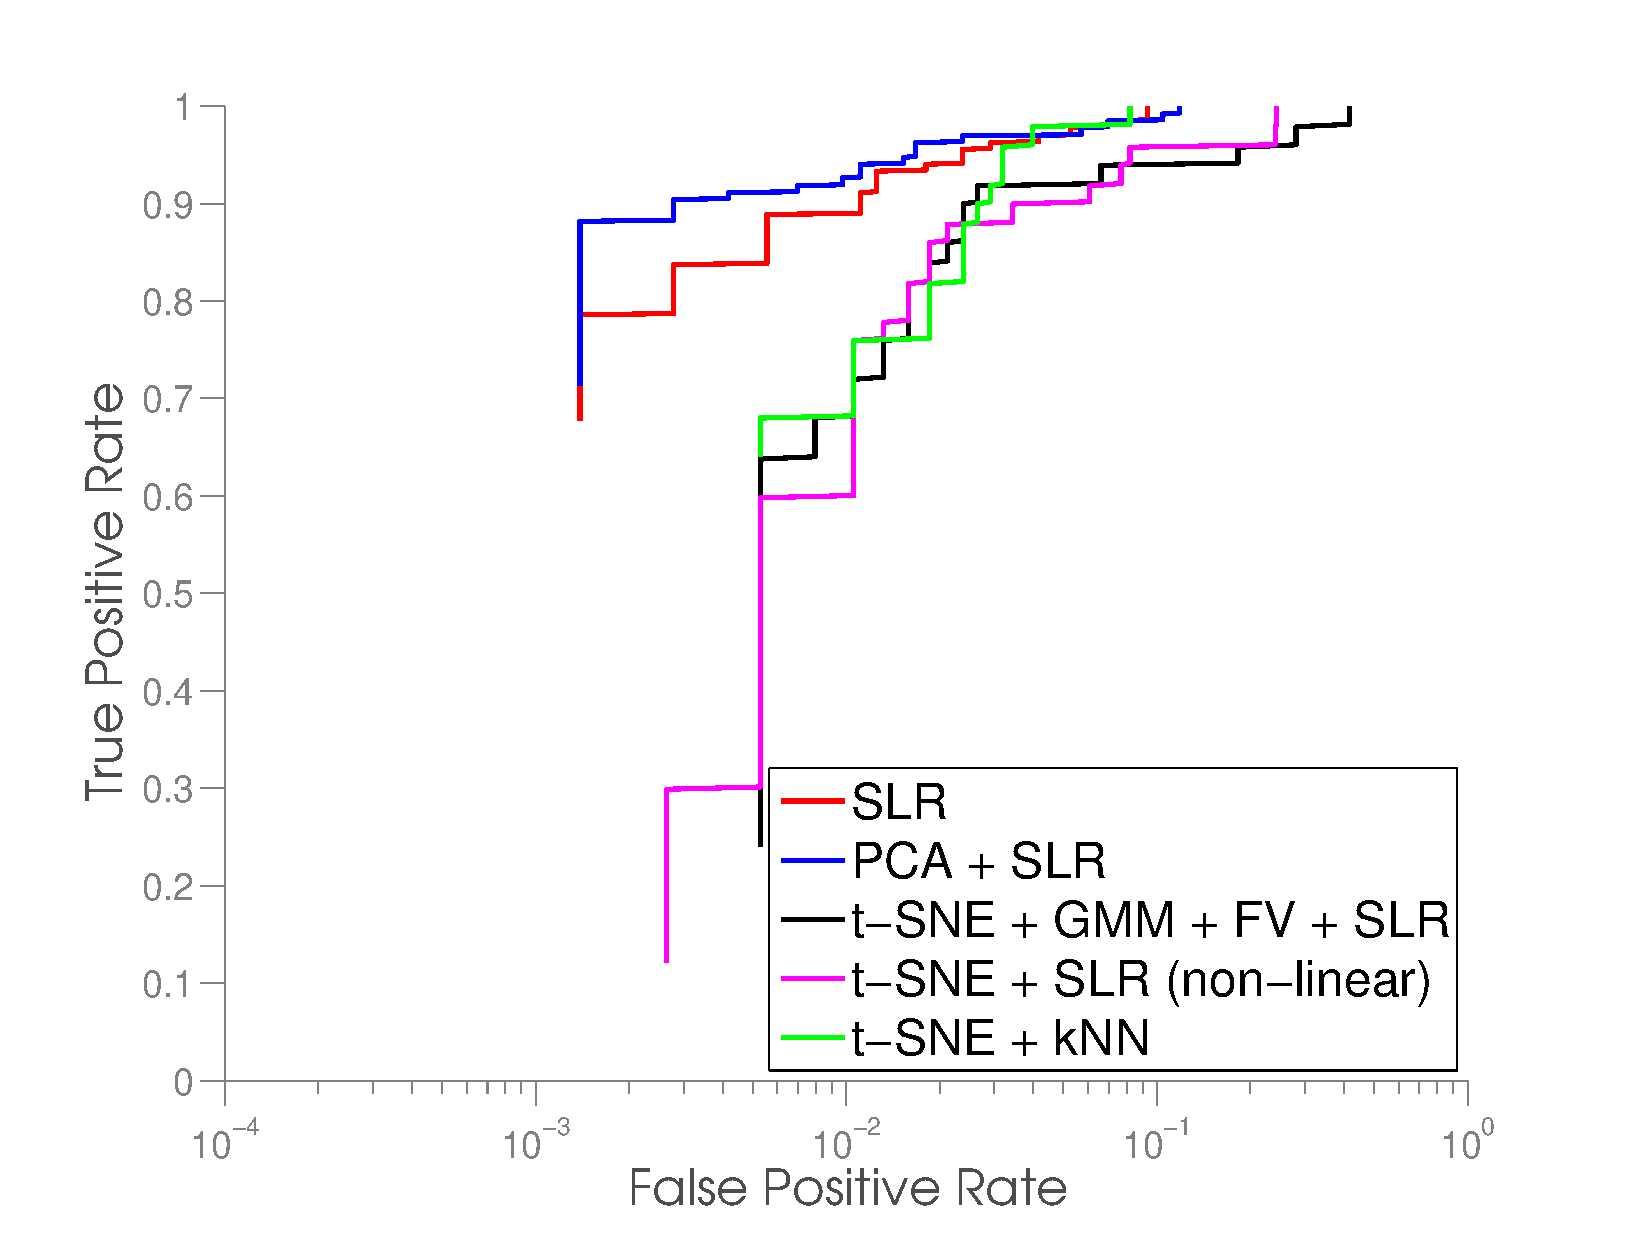
\includegraphics[trim=0mm 0mm
	6mm 10mm, clip=true,
	width=.475\columnwidth,height=4cm]{figures/ROC_all_methods.eps}
		\label{fig:ROCCurve}}
	\caption{Left: True vs Predicted values; Right: Average error for different
	user / item categories}
\end{figure}

\begin{figure}[!t]
	\center
	\subfigure[Error vs number of dimensions for PCA]
	{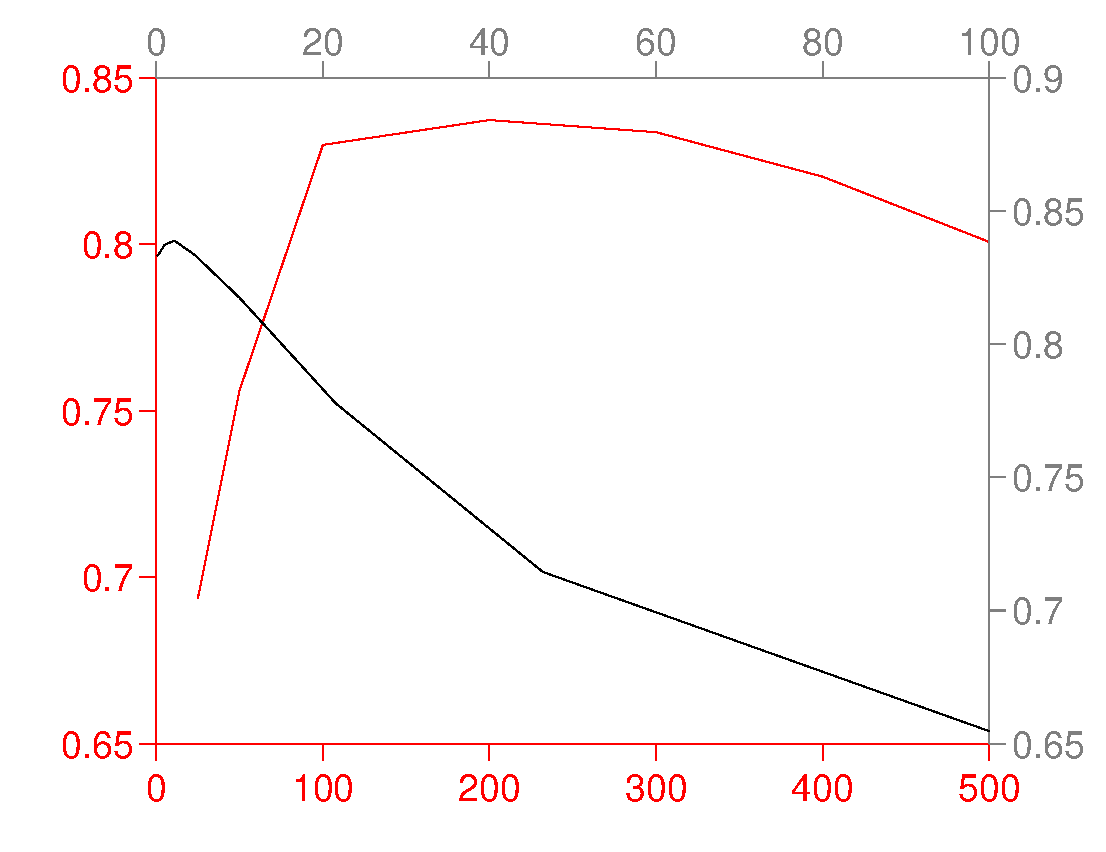
\includegraphics[trim=0mm 0mm 0mm 0mm, clip=true,
	width=.4\columnwidth]{figures/PCA_dim_and_lambda_val.eps}
	\label{fig:DimCurve}}
	\hfill
	% trim option's parameter order: left bottom right top
	\subfigure[Number of non-zero coeficients in SLR vs train-test ratio]
	{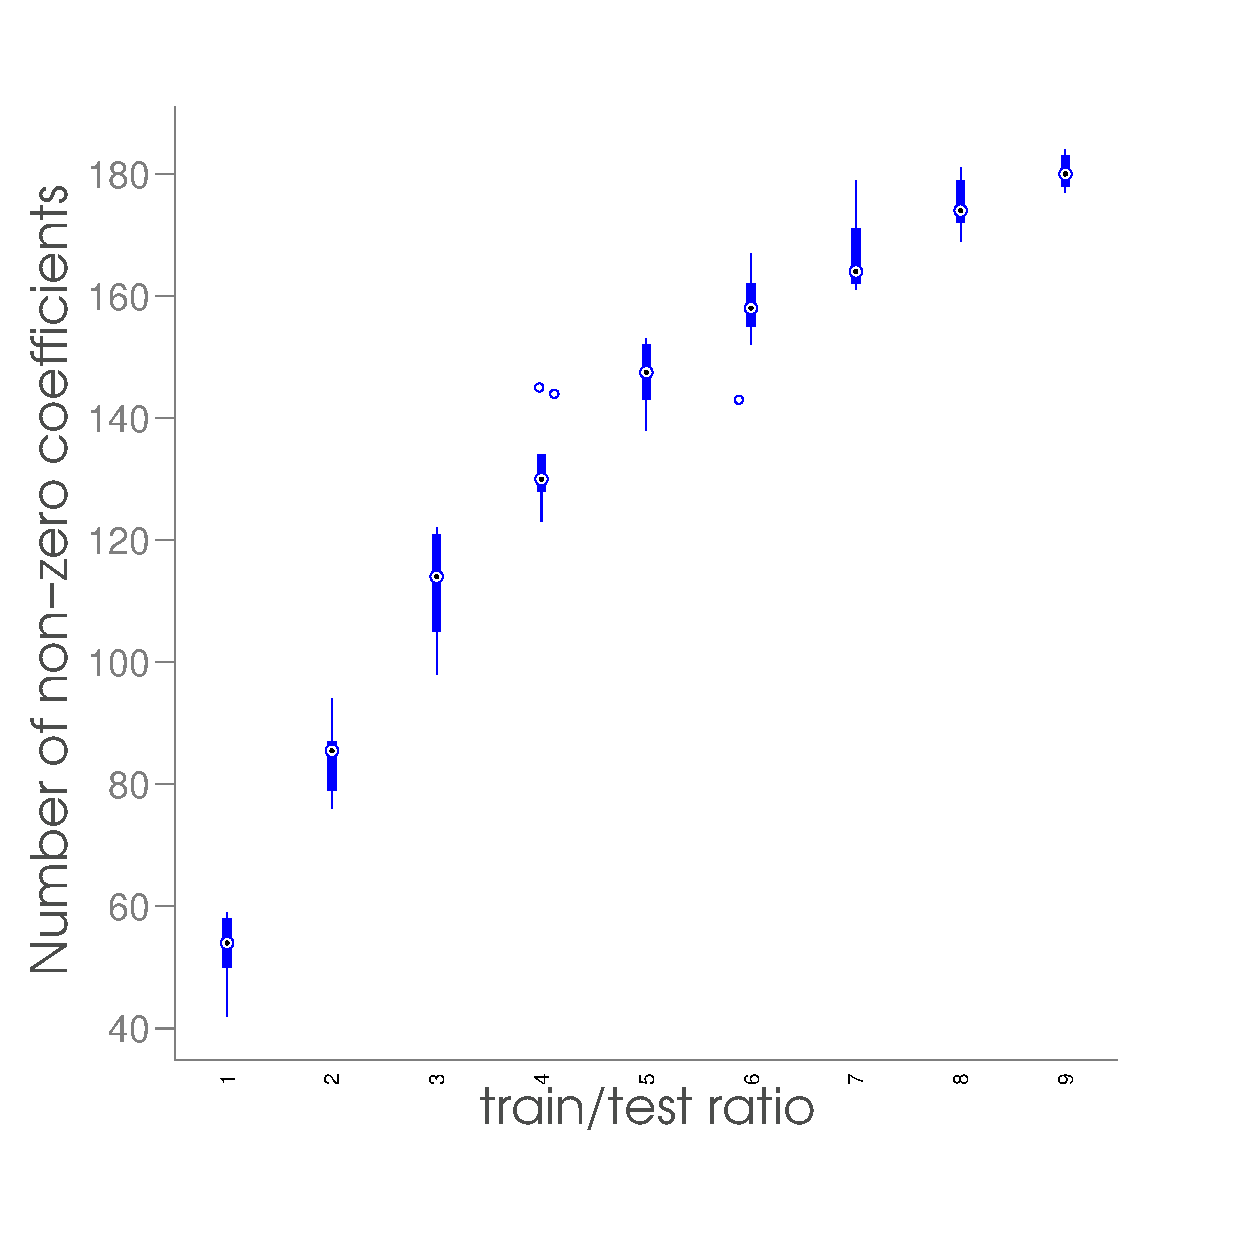
\includegraphics[trim=0mm 10mm 0mm 0mm, clip=true,
	width=.35\columnwidth]{figures/SMLR_used_coefficients.eps}
		\label{fig:NonZeroCurve}}
	\caption{Left: Error Vs number of PCA dimensions; Right: Number of non-zero
	coeficients in SLR based on the train-test ratio.}
\end{figure}


%Our simplest method 

Since the t-SNE mapping looks very natural for the human observer, 
we have tried to use it with classification methods. For that purpose, 
we first tried classifying the data samples with the simple kNN. 
With grid-search and 10-fold cross-validation, we have found that an optimal
number of neighbours is 7.
As it can be seen on Figure \ref{fig:ROCCurve}, this approach was not very
successful- our true-positive predictions are low 
when we choose to return only the samples for which we are certain that are a human. 
As we start to relax the threshold, we quickly start returning false positives, which pulls 
our ROC curve to the right of the plot.

A similar observation is valid for all methods which use the t-SNE for dimensionality reduction. 
When using a non-linear SLR for the classification we get almost the same ROC curve. 
We have also tried modelling the emission of our data with a Gaussian mixture model (GMM) by using 32 Gaussians.
 Then we computed the FV representation for each of our features, which leads to features having 128 dimensions.
  Although this approach is very widely used for image classification and segmentation, 
  in our case it performed on par with the previous two approaches (k-NN and non-linear SLR).
   We suspect that the problem for all three previous approaches, and thus their weak performance, 
   lies in the t-SNE mapping. Although it manages to group the positive samples fairly well, 
   it also introduces many negative samples in the same region. Using different transformation metrics 
   afterwards, or just applying classifiers both struggle with the negative samples which 
   bunch together with the positive samples, which push our ROC curve to the right.

Our best approach is based on computing the PCA transformation of the input data, and the classifying 
it with the SLR classifier. We used 10-fold cross-validation for determining the
optimal lambda from the range $10^{-1}$ to $10^{2}$. Also, we have used cross-validation to select the correct number of 
most important PCA dimensions. The pair of values which provided the best predictions 
are $\lambda = 2.9$ and $D = 250$. The prediction accuracy versus the number of PCA 
dimensions can be seen on Figure ???. When we use a small number of dimensions, they 
do not carry enough information about the signal, thus we have bad prediction accuracy. 
A similar statement can be made when we use too many dimensions, since they start to 
pollute the signal with measurement noise.

On Figure \ref{fig:ROCCurve}, we can see that this approach performs very well
even in the range of predictions with high confidence, i.e. it does not return many false positives. The 
sparsity of the space helps us to use the linear classifier, since at such a high 
dimensional space there can be found a hyperplane which splits the data
correctly.

It is interesting to see that the SLR works very well as a sparsity promoting classifier. 
On Figure ???, we show the number of non-zero weights for the 250 input features. 
As it can be seen, as more data is added to the training set, the more weights are used. 
This tells us that there is more information as the new features come. 
In addition, there is always a higher number of eliminated dimensions in the less 
important dimension, and more of the important dimensions are always kept, 
which is in line with what PCA does.

The learning curve for our best method is shown in Figure \ref{fig:LearnCurve}. As
expected, when we have little training data the prediction accuracy (average TPR) for the training set is high and 
for the test set is low, as we tend to over-fit. As more data is added to the train set, 
the prediction accuracy slightly decreases, however, the test accuracy increases considerably. 
From the variance of the errors we can see that the smaller datasets provide higher variance, 
since they are not a good representative of the global data set.

% <Learning curve for sparse logistic regression>(FIGURE). <Lambda curve>(FIGURE). 
% <PCA, different number of dimensions vs. prediction accuracy>(FIGURE). 
% <ROC curve. All algorithms>(FIGURE). 
% <2 worst misclassification pictures for pedestrians and not-pedestrians>(FIGURE)

\section{Implementation details}


\section{Conclusion}
In this work, we investigated several approaches for music recommendation and
image detection. For the music recommendation problem, KNN was our best
approach. However, we also found indications that we don't have enough training
data. With more data matrix factorization approaches could perform best. We have
also analyzed performance for different types of users and artist and provided
some insights into the data. For people detection problem, we found out that
combination of PCA and sparse logistic regression performs best. Additionally,
we were able to identify the most important features, as SLR solution promotes
sparsity. The results of t-SNE, altough appealing to the human eye, turned out
to be worse for this dataset.
	

\bibliographystyle{alpha}
\bibliography{document}

\end{document}